\chapter{Diseño}
\label{cap:capitulo4}

En este capítulo se expone, de forma detallada, el proceso seguido para conseguir que un dron detecte y navegue hacia una señal \ac{RF}.\\

Además, se muestra el desarrollo de una aplicación responsiva, que simula el comportamiento de una señal (en un espacio libre de obstáculos), basada en la aproximación de Friis.\\

Por último, se determina cuál de los métodos empleados es mejor y por qué, a través de diversas métricas comparativas.\\

A continuación, se puede observar un diagrama de bloques donde se ve una vista general del sistema empleado:\\

(METER DIAGRAMA DE BLOQUES)\\

\section{Preparación del entorno}
\label{sec:preparacion_del_entorno}

Inicialmente, se pone en funcionamiento el entorno de simulación (compatible con \ac{ROS}), así como el sistema de control de versiones, para mantener la trazabilidad y los backups. Por ello, se crea un repositorio común en GitHub y se instala y prueba el paquete de herramientas dispuesto por JdeRobot.

\subsection{JdeRobot - drones}
\label{subsec:jderobot_drones}

Gracias a esta plataforma, se obtienen los modelos y los módulos necesarios para simular en Gazebo 11 el desempeño de un cuadracóptero, provisto de un sistema autopilot PX4.\\

Específicamente, el modelo usado es el 3DR Iris simulado, con un plugin de una cámara frontal. Este dispositivo utiliza MAVROS para realizar la comunicación, lo que nos permite enviar y recibir mesajes ROS compatibles con el protocolo de comunicaciones típico de estas aeronaves, MAVLink.\\

\begin{figure} [H]
	\begin{center}
	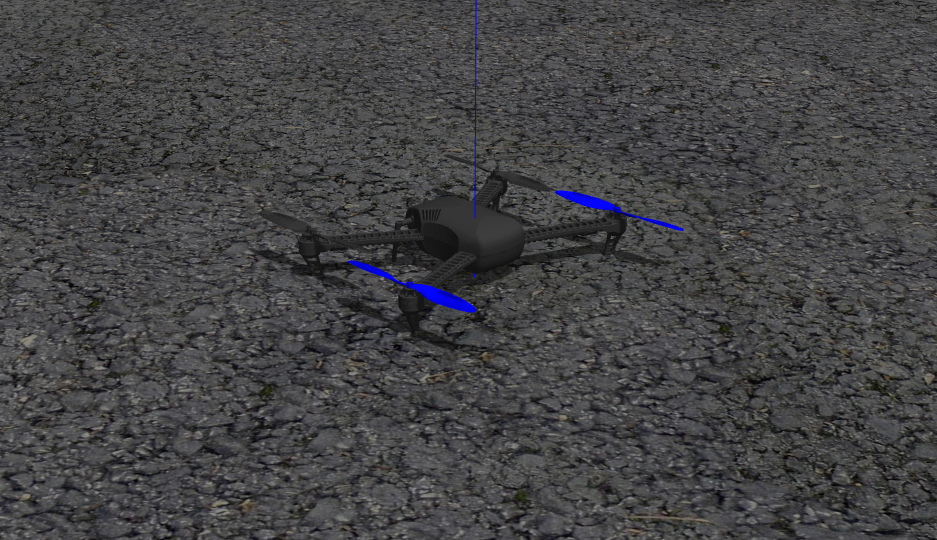
\includegraphics[height=4cm]{imagenes/cap4/1_px4_drone_gz.png}
	\end{center}
	\caption[3DR Iris simulado]{3DR Iris simulado}
	\label{fig:3dr_iris}
\end{figure}

\subsection{Teleoperador}
\label{subsec:teleoperador}

Una vez es funcional el entorno y los modelos, la primera aproximación ha consistido en realizar una interfaz gráfica simple, para enviar órdenes a la aeronave.\\

Para ello, se debe conseguir enviar mensajes de forma programática. Por tanto, se diseña un script controlador encargado de la comunicación directa con el controlador de la aeronave, que a su vez se encarga enviar y recibir diversos datos vía MAVROS. De igual modo, se satisfacen una serie de requisitos para asegurar el correcto funcionamiento del sistema:

\begin{enumerate}
	\item La comunicación se debe dar a más de 2 Hz, para evitar cambios indeseados en el funcionamiento interno del controlador PX4 (de la aeronave).

	\item Antes de realizar cualquier comunicación, se debe asegurar que el estado es \emph{``connected''}, lo que significa que el dron esta armado y en modo \emph{OFFBOARD} (nuestra aeronave posee 7 modos distintos, \emph{HOLD}, que mantiene la posición, \emph{RETURN}, que vuelve al punto de despegue, \emph{MISSION}, que permite cargar rutas programadas con anterioridad, \emph{TAKEOFF}, habilita el despegue, \emph{LAND}, habilita el aterrizaje, \emph{FOLLOW ME}, que permite seguir objetivos, y \emph{OFFBOARD}, que permite comandar al dron sin necesidad de GPS, lo que es útil de cara al desarrollo de aplicaciones robóticas) \cite{flight-modes}.

    \item Una vez está conectado, se deben enviar datos (velocidades en nuestro caso) al controlador PX4, con el fin de evitar el cierre de la conexión. Estos datos carecen de utilidad más que la de asegurar dicha conectividad.

    \item Por último, y antes de enviar cualquier posición, velocidad o comando (distintos modos de actuación), se debe comprobar siempre que el modo activo es \emph{OFFBOARD} y que el dron esta armado (listo para volar). En caso contrario, se debe solicitar al controlador, mediante servicios, dichos requerimientos.
\end{enumerate}

Por tanto, la manera de generar comportamientos en el dron en sí, es mediante \emph{topics}. Concretamente, los que genera MAVROS automáticamente cuando se lanza todo el sistema. Tal y como se comentó en apartados anteriores, estos \emph{topics} sólo admiten mensajes \ac{ROS}, lo que encapsula el mensaje real transmitido al controlador PX4, que solo es compatible con MAVLINK.\\

En nuestro caso, se envían posiciones (PoseStamped), velocidades (Twist) y comandos (sevicios formados por mensajes personalizados, creados por MAVROS, con formato \ac{ROS}). Esto, nos permite conectar el resto de aplicaciones con el script controlador, mediante \emph{topics} comunes, de forma de que el script controlador se encargue de enviar la acción final al dron, mientras el resto de scripts se encarguen de resolver otras tareas.\\

De este modo, el teleoperador se diseña con el fin de generar comportamientos que se usarán en las fases finales del \ac{TFG}. Sin embargo, para la primera versión, tan solo se construye una interfaz gráfica sencilla, encargada de enviar ordenes usando \ac{ROS} que, en última instancia, llegan al dron y producen diversos comportamientos, tales como moverse y girar, a través de barras de acción.\\

\begin{figure} [H]
	\begin{center}
	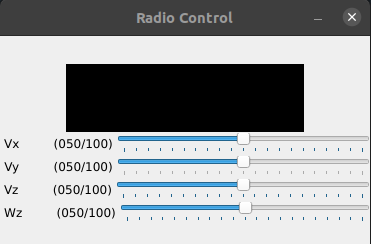
\includegraphics[height=4.5cm]{imagenes/cap4/2_axes_rc.png}
	\end{center}
	\caption[Primera versión del teleoperador]{Primera versión del teleoperador}
	\label{fig:teleoperador_v1}
\end{figure}

En la siguiente versión, se programan comportamientos predefinidos, es decir, acciones predeterminadas tales como desplazarse distancias concretas en ciertas direcciones, o girar un número específico de grados en un sentido u otro. Para ello, se diseña una ampliación sobre la interfaz anterior, en la que se añade un botón por cada acción concreta desarrollada, además de una imagen de la cámara frontal en tiempo real.\\

Por últmo, se afina el comportamiento de las acciones predefinidas, para hacer que el dron se desplazase de celda en celda, concretamente de centro en centro. La idea de esto es que, el dron solo podrá tomar medidas de la señal en posiciones concretas y no en movimiento. Además, se agregan marcadores en \emph{rviz}, para determinar las celdas visitadas (con colores aleatorios), junto con otro marcador que muestra la trayectoria que sigue la aeronave.\\

\begin{figure} [H]
	\begin{center}
	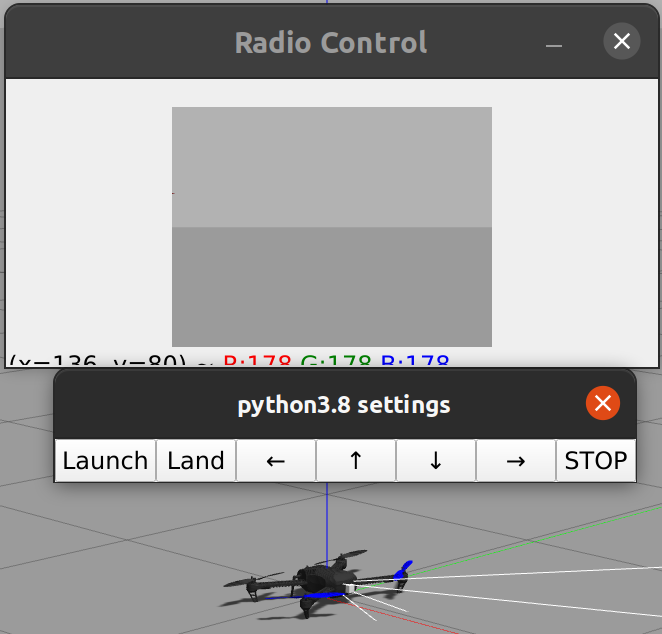
\includegraphics[height=8cm]{imagenes/cap4/3_c2c_gui.png}
	\end{center}
	\caption[Versión final del teleoperador]{Versión final del teleoperador}
	\label{fig:teleoperador_end}
\end{figure}

A continuación, se muestra el \emph{``main''} de la aplicación mencionada:\\

\begin{code}[H]
\begin{lstlisting}[language=Python]
if __name__ == '__main__':
    try:
        rospy.init_node(NODENAME, anonymous=True)

        # Msgs
        ## Subscribers
        image_sub = rospy.Subscriber(IMAGE_TOPIC, Image, callback = image_cb)
        current_pos_sub = rospy.Subscriber(LOCAL_POSE_TOPIC, PoseStamped, callback = current_pos_cb)

        ## Publishers
        pos_pub = rospy.Publisher(RADIO_CONTROL_POS_TOPIC, PoseStamped, queue_size=10)
        cmd_pub = rospy.Publisher(RADIO_CONTROL_CMD_TOPIC, Px4Cmd, queue_size=10)

        # -- OPENCV -- #
        cv2.namedWindow(WINDOWNAME)

        # Buttons
        cv2.createButton('Launch', launch_button, None, cv2.QT_PUSH_BUTTON, 1)
        cv2.createButton('Land', land_button, None, cv2.QT_PUSH_BUTTON, 1)
        cv2.createButton('←', left_button, None, cv2.QT_PUSH_BUTTON, 1)
        cv2.createButton('↑', front_button, None, cv2.QT_PUSH_BUTTON, 1)
        cv2.createButton('↓', back_button, None, cv2.QT_PUSH_BUTTON, 1)
        cv2.createButton('→', right_button, None, cv2.QT_PUSH_BUTTON, 1)
        cv2.createButton('STOP', stop_button, None, cv2.QT_PUSH_BUTTON, 1)

        cv2.waitKey(0)
        cv2.destroyAllWindows()
    except rospy.ROSInterruptException:
        pass
\end{lstlisting}
\caption[Main de center to center app]{Main de center to center app}
\label{cod:c2c_app}
\end{code}

Donde, tras inicializar el nodo \ac{ROS}, se definen por un lado los suscriptores, encargados de recibir los datos de la cámara y la posición del dron (usando MAVROS), los publicadores, cuya función es enviar posiciones y/o comandos al script controlador, y por último la interfaz gráfica diseñada con OpenCV, donde se define la ventana y los botones con las diversas acciones predefinidas \footnote{Código completo en \url{https://github.com/RoboticsLabURJC/2022-tfg-cristian-sanchez/blob/main/src/teleop/scripts/c2c_control.py}}.\\

\section{Modelo de propagación de señal}
\label{sec:signals}

El siguiente paso consiste en generar un modelo de propagación de señales \ac{RF}. Este apartado es especialmente relevante, ya que nos permite desarrollar una aplicación reactiva, con la idea de generar entornos en tiempo real, sobre los que probar nuestras soluciones.\\

Pero, antes de entrar en detalle en estos aspectos, conviene familiarizarse con algunos conceptos básicos sobre el procesamiento de señales:

\begin{enumerate}
	\item \emph{Señal}: se trata de una función que describe un fenómeno físico, y que se emplea para la transmisión de información.

    \item \emph{Dominio temporal}: establece el eje de abcisas con el tiempo.

    \item \emph{Dominio de la señal}: determina si la señal se expresa en tiempo o en frecuencia (a través de transformadas).

    \item \ac{ADC}: elemento electrónico que permite la conversión de señales analógicas a señales digitales.

    \item \ac{RSSI}: permite establecer el nivel de potencia de una señal, con respecto a 1 mW de potencia. Se expresa en dBm.

    \item \ac{SNR}: métrica que permite medir la potencia de la señal con respecto al ruido ambiente.

    \item \emph{Frecuencia}: parámetro de la función que define a la señal, el cual determina el número de veces que se repite en un segundo. Se mide en hercios (Hz).

    \item \emph{TX}: Se refiere a la transmisión de la señal.

    \item \emph{RX}: Hace referencia a la recepción de la señal.
\end{enumerate} \cite{basics-signals}\\

En cuanto al modelo de propagación de señal, se puede definir como un sistema capaz de calcular de que manera comporta la potencia de una señal, según las características de su entorno.\\

\subsection{Aproximación de Friis}
\label{subsec:friis}

Por ello, se opta por emplear la aproximación de Friis, que nos proporciona una ecuación para  modelizar nuestro problema:

\begin{align}
    P_r = P_t \cdot \left( \frac{G_t G_r \lambda^2 }{(4 \pi)^2 d^n L} \right)
\end{align}

Donde cada término significa lo siguiente:

\begin{enumerate}
    \item \emph{$P_t$ y $P_r$}: aluden a la potencia del transmisor y la potencia del receptor respectivamente.

    \item \emph{Ganancias} ($G_t$, $G_r$): representan un valor incremental aplicado a la potencia de emisión y de recepción, respectivamente.

    \item \emph{Valor lambda} ($\lambda$): hace referencia a la longitud de onda. Está directamente relacionado con la frecuencia.

    \item \emph{Distancia} (d): desde el origen de la señal a un punto en el espacio.

    \item \emph{L}: representa todas aquellas pérdidas no asociadas a la propagación de la señal.

    \item \ac{PLE} (n): permite ajustar el modelo a diversos entornos. Es un valor constante extraido de forma empírica. A continuación se muestra una tabla con varios ejemplos.
\end{enumerate} \cite{friis-1}\\

\begin{figure} [H]
	\begin{center}
	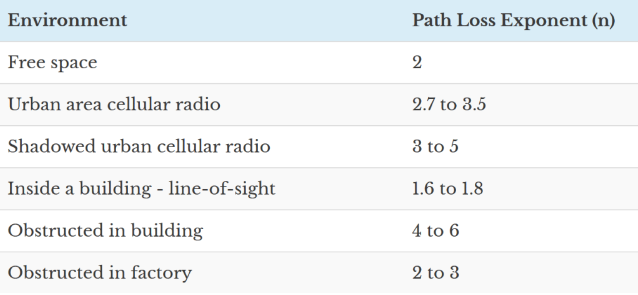
\includegraphics[height=5cm]{imagenes/cap4/4_PLE_table.png}
	\end{center}
	\caption[Tabla ejemplos exponente n]{Tabla ejemplos exponente n}
	\label{fig:ple_table}
\end{figure}

Además, empleando este método, podemos modelizar las pérdidas de una señal estimadas durante su propagación, a través de la siguiente ecuación:\\

\begin{align}
    P_L(dB) = -10 \log_{10} \frac{\lambda^2}{(4 \pi d)^2}
\end{align}

Sin embargo, para nuestro caso no es relevante (aunque se incluye dentro del módulo).\\

\subsection{Módulo python de Friis}
\label{subsec:friis-module}

Una vez desarrollado lo anterior, lo siguiente consiste en encontrar la forma de que todo esto sea accesible para cualquier aplicación que lo desee.\\

Por ello, surge la idea de crear un módulo python encargado de modelizar las ecuaciones previamente mencionadas. Para ello, se diseña una clase cuyo constructor recibe, por parámetros, las variables implicadas en las ecuaciones de Friis, además de las dimensiones del mapa y su resolución (la cual afecta al tamaño de celda).\\

Básicamente, el proceso a seguir para usar este módulo es el siguiente, primero se crea un objeto de la clase Friis donde se especifican las características de la señal y las variables relacionadas con el mapa, lo que genera internamente un array 2D vacío, que será rellenado en función del modelo seleccionado. Posteriormente, se selecciona el modelo deseado (propagación o pérdidas, este último no está testeado), pasando las coordenadas del origen de la señal por parámetros. Esto, retornará el mapa relleno con los valores asociados a las ecuaciones del modelo de Friis seleccionado.\\

A continuación se muestra un ejemplo sencillo de uso, donde se obtiene un mapa de propagación de señal, en forma de Numpy array 2D:

\begin{code}[H]
    \begin{lstlisting}[language=Python]

    #! /usr/bin/env python
    import friss as fr

    if __name__ == '__main__':
        friis_object = fr.Friss(power_tras=10.0,
                                gain_tras=1.5,
                                gain_recv=2.0,
                                freq=fr.FREQ_WIFI,
                                losses_factor=1.0,
                                losses_path=2.0,
                                world_sz=(10,10),
                                resolution=1.0)

        signal_map = friis_object.model_power_signal(origin=(5,3))

\end{lstlisting}
\caption[Ejemplo básico de uso del módulo Friis]{Ejemplo básico de uso del módulo Friis}
\label{cod:friis_basics}
\end{code}

Concretamente, se genera un mapa 10x10 con resolución 1 (es decir, cada celdilla es de 1x1 unidades), de una señal WIFI, donde el transmisor emite a 10 W, con una ganancia de 1.5, el receptor posee una ganancia de 2, un factor de pérdidas (L) de 1, es decir, sin pérdidas, y por último, el exponente n (\ac{PLE}) con un valor de 2, que representa el espacio vacío. Luego se genera el mapa de propagación de la señal, indicando que la fuente se encuentra en las coordenadas (5,3).\\

No obstante, este módulo posee otras funcionalidades útiles para trabajar con él, como son:

\begin{enumerate}
    \item \emph{reset\_world}: modifica el mapa que hubiera, estableciendo todos sus valores a cero.

    \item \emph{get\_world\_sz}: retorna las dimensiones del mapa.

    \item \emph{set\_values}: modifica las características de la señal simulada.
\end{enumerate}

Hay que tener en cuenta que, aunque se modifiquen los parámetros, se debe modelar de nuevo el mapa para que surtan efectos los cambios.\\

\subsection{Aplicación de Friis}
\label{subsec:friis-app}

Finalmente y agrupando lo anterior, se integra el módulo previo, en una interfaz gráfica intuitiva para el usuario. La idea es estudiar, en tiempo real, como evoluciona la señal cuando alguno de sus parametros, en la ecuación de Friis, es modificado.\\

Para ello, se emplea la librería matplotlib, debido a la enorme cantidad de herramientas de las que dispone, así como de su sencillez a la hora de crear nuevas aplicaciones. Funciona de manera que se generan eventos que son gestionados en \emph{``callbacks''}, es decir, se generan bucles asociados a dichos eventos, que reaccionan a cambios en la interfaz generada.\\

En nuestro caso, la estructura base consta de una figura, sobre la que se agregan todos los elementos, entre los que encontramos los mapas de calor o \emph{``heatmap''} en forma de plots, las barras de acción o \emph{``sliders''}, botones, entre otros elementos que se explicarán más adelante.\\

Inicialmente, se opta por representar un mapa de calor con una barra de color asociada a los distintos valores de la señal. Además, se integran sliders correspondientes a cada valor presente en la ecuación de Friis, tal y como se muestra a continuación:\\

\begin{figure} [H]
	\begin{center}
	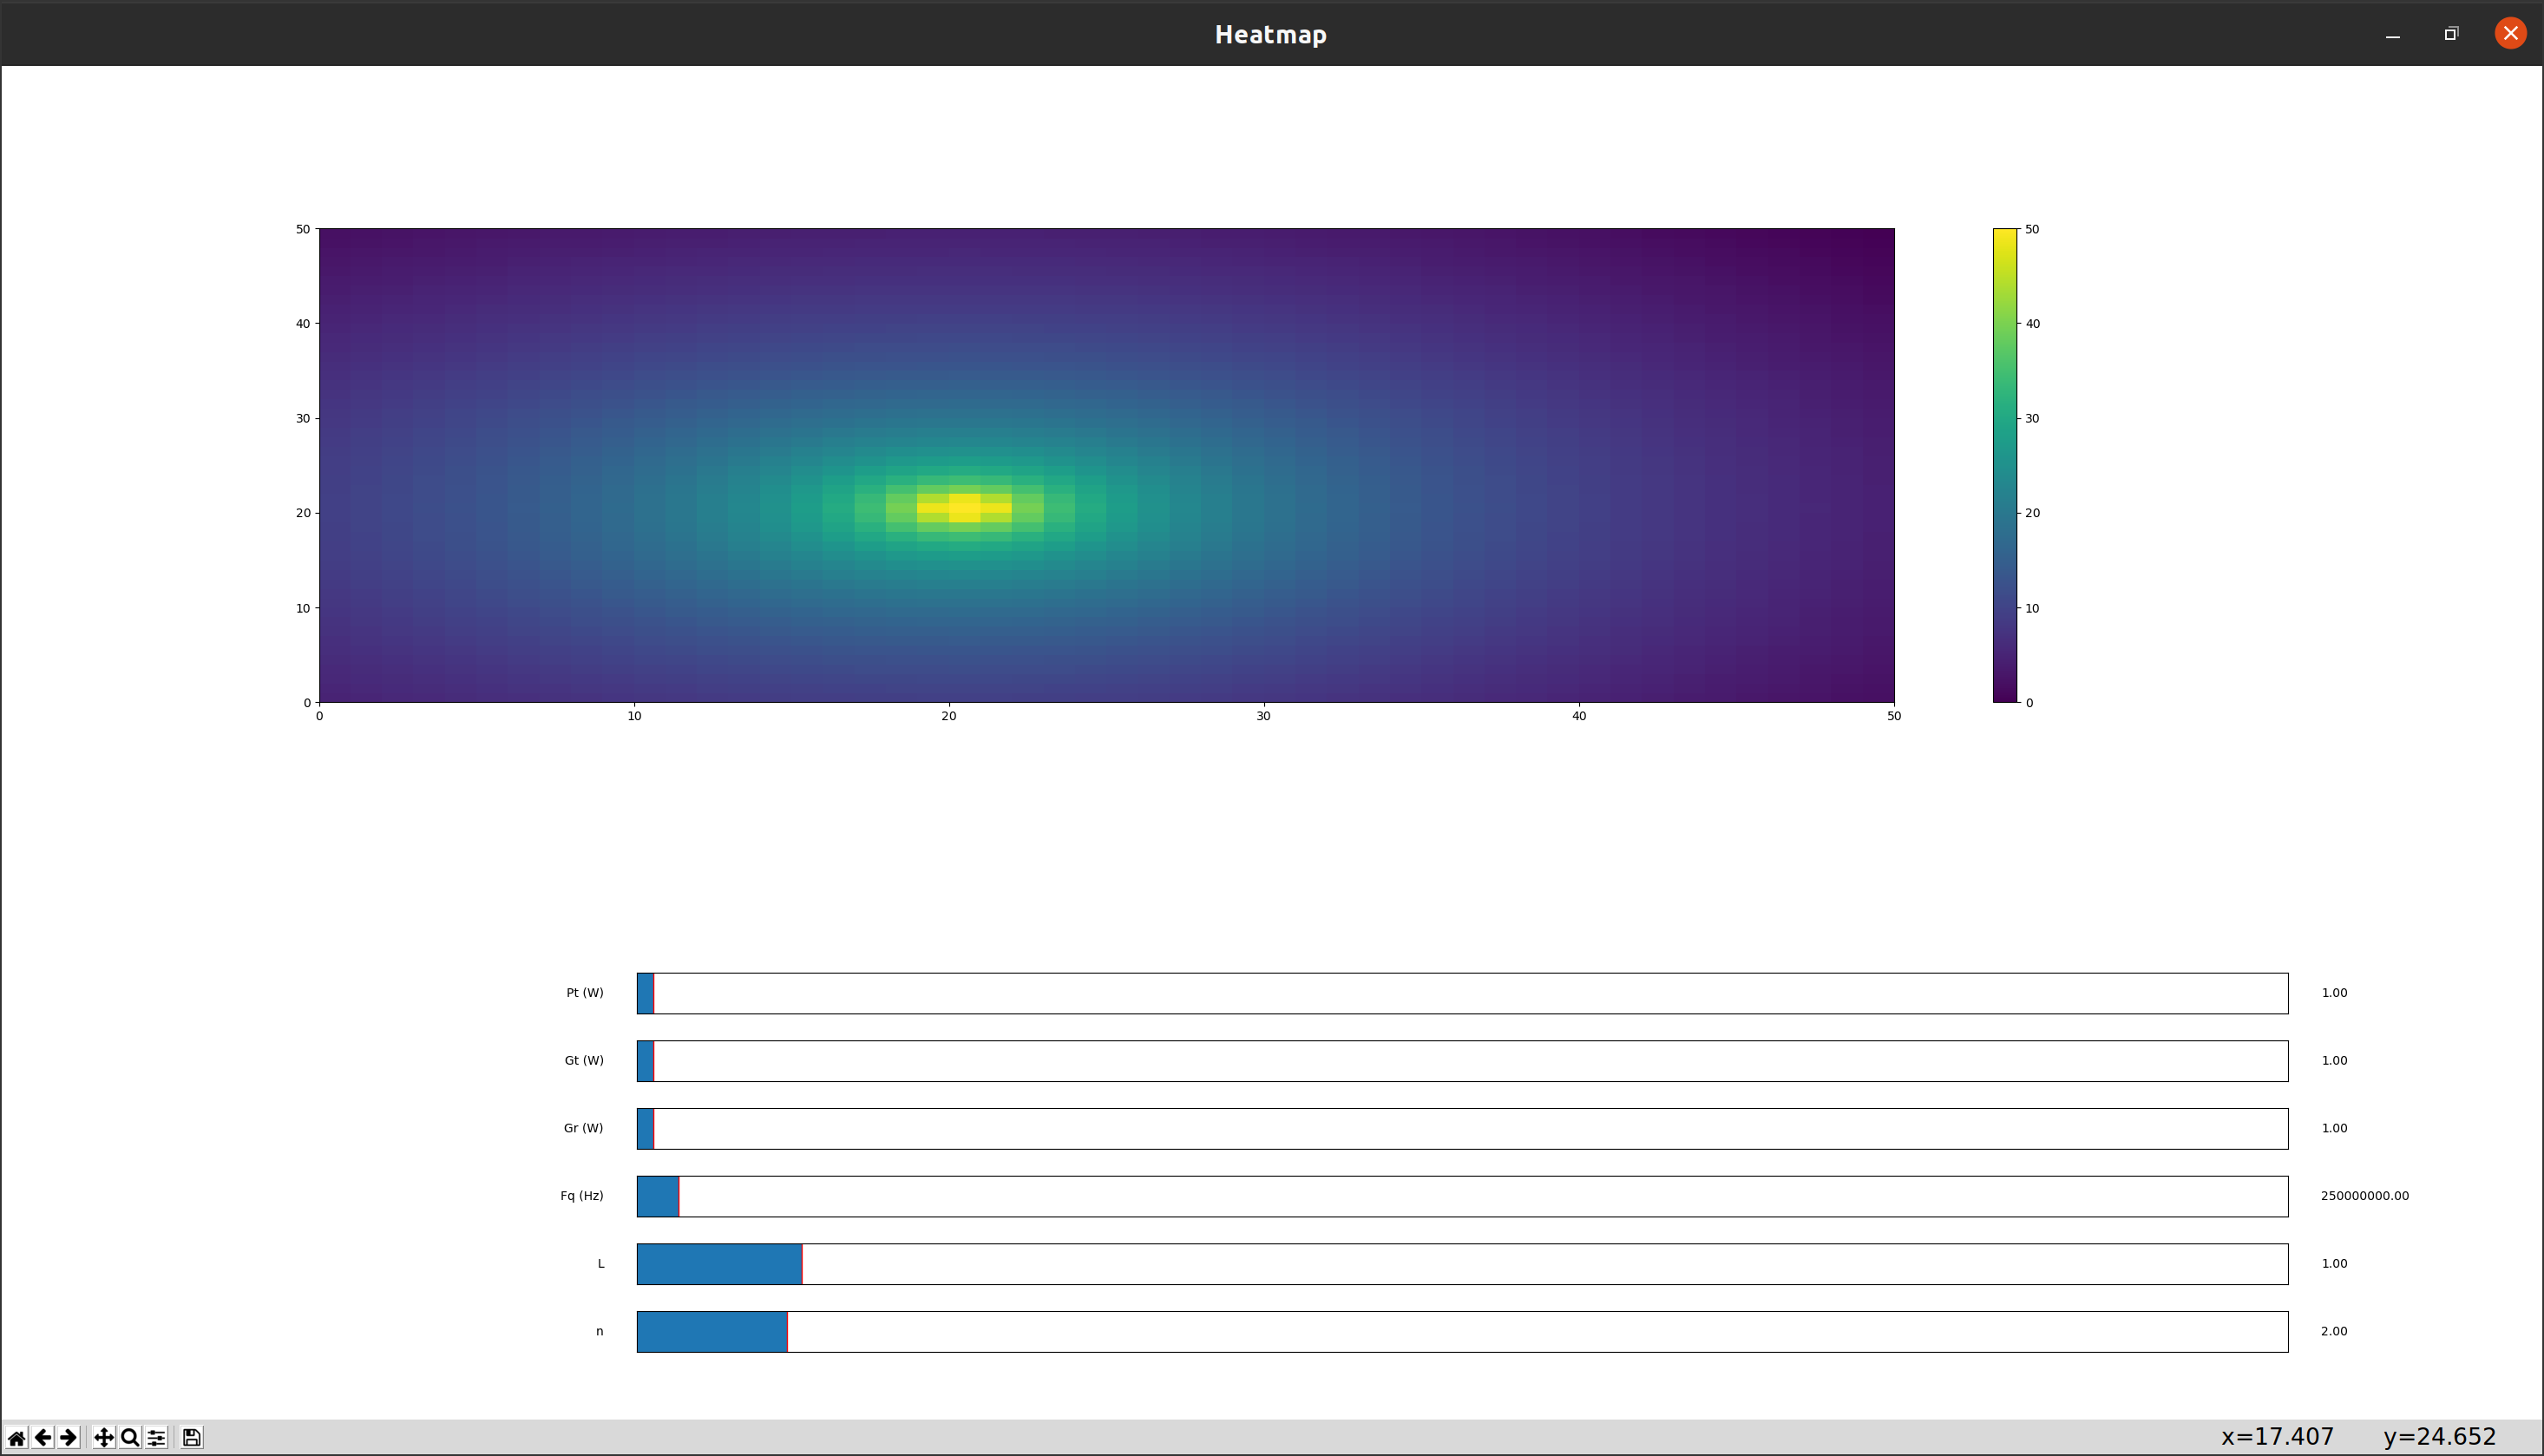
\includegraphics[height=7cm]{imagenes/cap4/6_Friss_firstGUI.png}
	\end{center}
	\caption[Primera versión de la interfaz]{Primera versión de la interfaz}
	\label{fig:friis_init_app}
\end{figure}

El problema es, que al actualizar los valores, también lo hace la representación, por lo que no se aprecia el efecto de los cambios en el plot.\\

Por ello, se decide agregar dos mapas de calor, uno con el máximo y el mínimo fijados a mano (donde sí se aprecian los cambios), y el anterior mencionado. Para elegir cual usar, se añade una casilla marcable. Además, se incluyen dos variables relevantes a la hora de modelar, el tamaño del mapa y la resolución, manejadas a través de \emph{``sliders''}, los cuales a su vez se activan al pulsar un botón de SET, que recarga la interfaz. Además, se ajustan los saltos de valores para que sean coherentes en el resto de barras de acción, tal y como se puede apreciar a continuación:\\

\begin{figure} [H]
    \begin{center}
    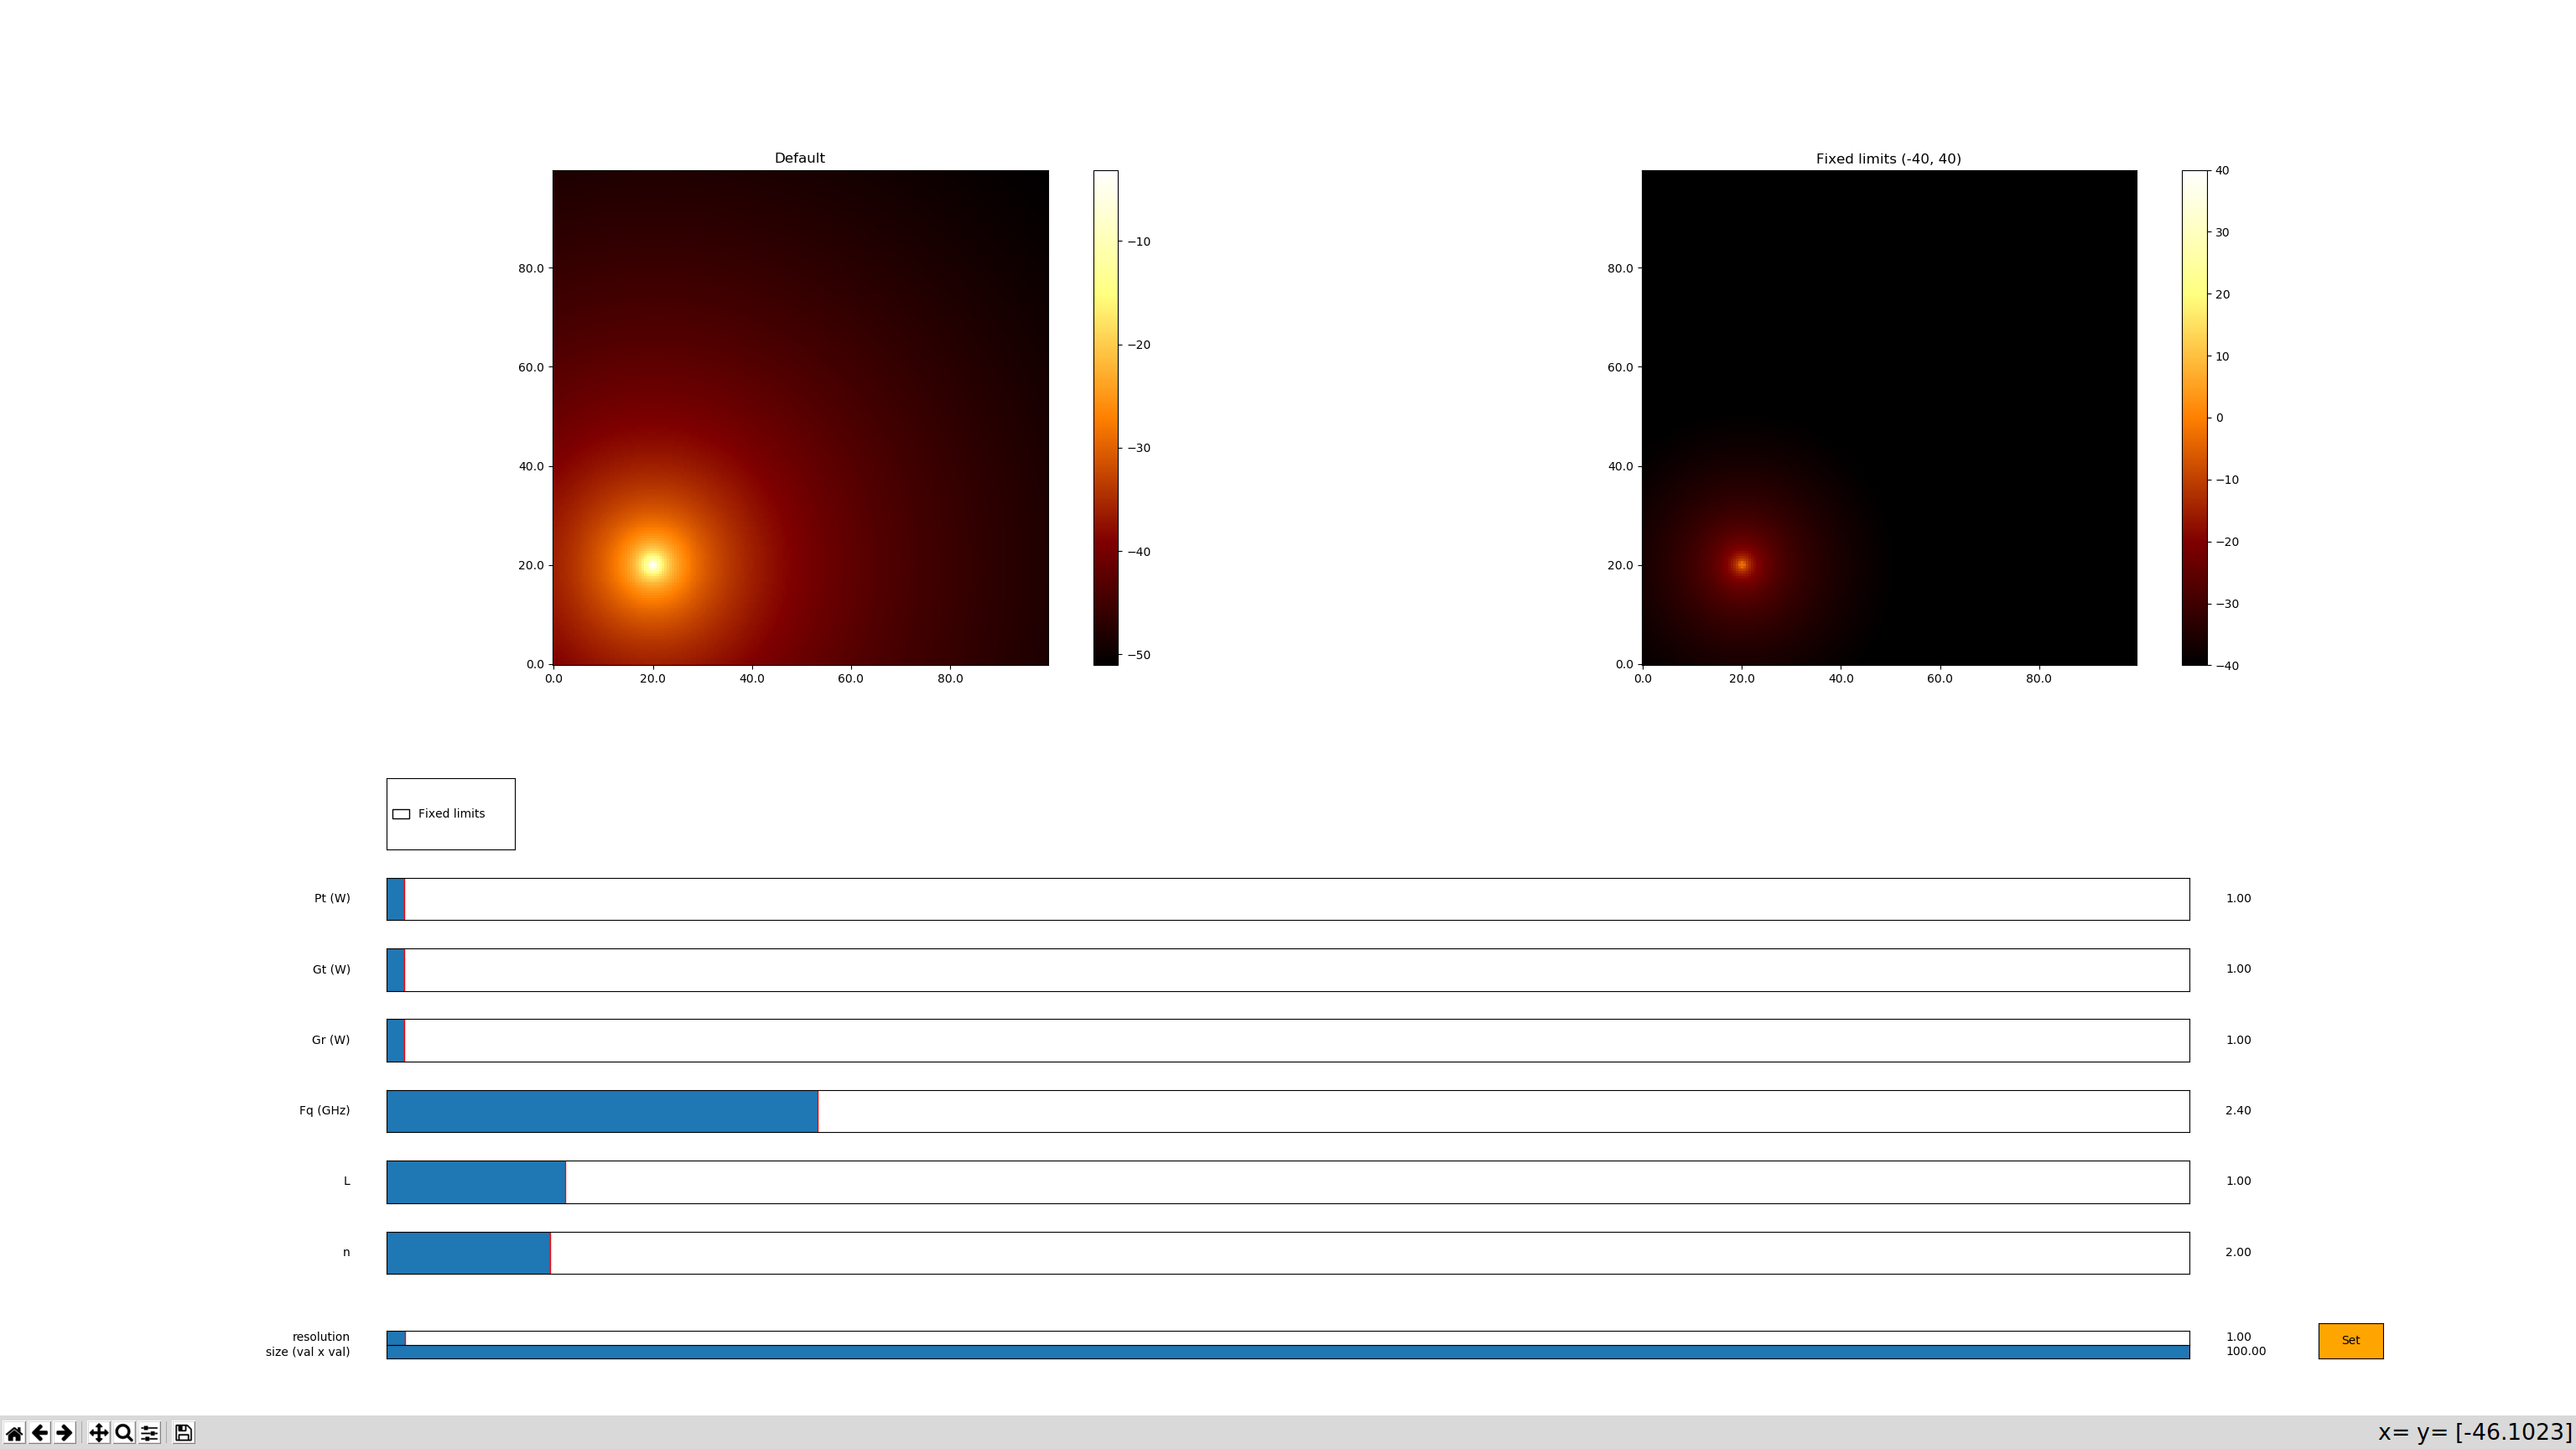
\includegraphics[height=8cm]{imagenes/cap4/7_Friss_endGUI.png}
    \end{center}
	\caption[Versión final de la interfaz]{Versión final de la interfaz}
	\label{fig:friis_end_app}
\end{figure}

Cabe destacar que, por motivos de desarrollo, no se ha añadido la parte de generación dinámica de obstáculos a la aplicación, ya que esta planteó como un extra al final del \ac{TFG}.\\

\section{Comportamiento sigue señal basado en \ac{RF}}
\label{sec:signal_follow}

\subsection{Introducción al problema}
\label{subsec:intro_sf}

El problema a resolver en este caso, es el de detectar y navegar hacia una señal, empleando diversos algoritmos, para compararlos posteriormente. Por consiguiente, se ha realizado una integración conjunta de todos los puntos mencionados anteriormente.\\

Para ello, se ha diseñado una aplicación servidor de datos, que funciona como intermediaria con el módulo de Friis. Siendo concisos, dicha aplicación contiene dos servidores basados en acciones \ac{ROS}, que son especialmente útiles en este caso, dada su naturaleza asíncrona. Dichos servidores gestionan las peticiones para el dron y para rviz, tal y como se cuenta a continuación:

\begin{enumerate}
	\item \emph{Caso dron}: en términos generales, el dron envía su posición en coordenadas transformadas al sistema de referencia del \emph{``heatmap''}, y recibe el valor de la señal de dichas coordenadas. En un caso real, el dron tan solo accedería al valor de la señal a través de un sensor que se lo permitiera. Además, se le ha agregado la funcionalidad de enviar, en dicha petición, si se deseaba un mapa con obstáculos o no, para compatibilizar el funcionamiento con entornos dinámicos.

	\item \emph{Caso rviz}: recibe una petición donde se agregan todas las características de la señal para generar el \emph{``heatmap''} deseado, vease el origen y sus componentes. Esto, genera como respuesta un array de floats que contienen la información del mapa de calor, en un formato adecuado para su representación, es decir, para generar el mapa de forma gráfica, se emplea la biblioteca grid\_map, que a través de un topic de \ac{ROS}, permite enviar los datos a un plugin de rviz, el cual genera la representación visual buscada\footnote[2]{Toda la funcionalidad englobada en el directorio heatmap\_util del proyecto}. También ha sido agregada la funcionalidad de los obstáculos para la experimentación futura.
\end{enumerate}

\subsection{Algoritmos}
\label{subsec:algoritmo_sf}

Antes de definir los algoritmos empleados, lo primero es determinar la base de la que se ha partido para desarrollarlos.\\

Por ello, inicialmente se ha definido una clase \emph{``Drone''}, cuyo constructor se encarga de conectar los topics al controlador PX4 para comandar ordenes a la aeronave. Además, se encarga de establecer la comunicación con el servidor de datos (tanto para la potencia como para rviz) y define los diferentes atributos pertenecientes a la clase, que en este caso aluden a los parámetros necesarios para el funcionamiento de los algoritmos y la extracción de datos en los resultados.\\

En general, la clase sigue la siguiente estructura:

\begin{enumerate}
	\item \emph{Métodos para comandar al dron}: que se definen como el conjunto de funciones encargadas del movimiento del dispositivo (como despegar, aterrizar, desplazarse, entre otros). Mucha de esta funcionalidad ha sido adaptada del teleoperador comentado al de este capitulo.

    \item \emph{Métodos de tolerancia}: encargados de establecer un margen aceptable entre la posición del dron y el objetivo deseado. Estos métodos permiten controlar con precisión problemas que surgen de la deriva y de condiciones externas, como puede ser el viento.

	\item \emph{Métodos de conversión}: que permiten transformar las coordenadas entre los distintos sistemas de referencia presentes en el problema, tal y como se puede apreciar a continuación.

    \item \emph{Algoritmos}: o las soluciones \emph{``sigue señal''} propiamente dichas, que en sí, contienen el conjunto de métodos que cada cual necesita para llevarse a cabo. Se puede distinguir entre manual, manual optimizado y Q-Learning.
\end{enumerate}

\begin{figure} [H]
    \begin{center}
    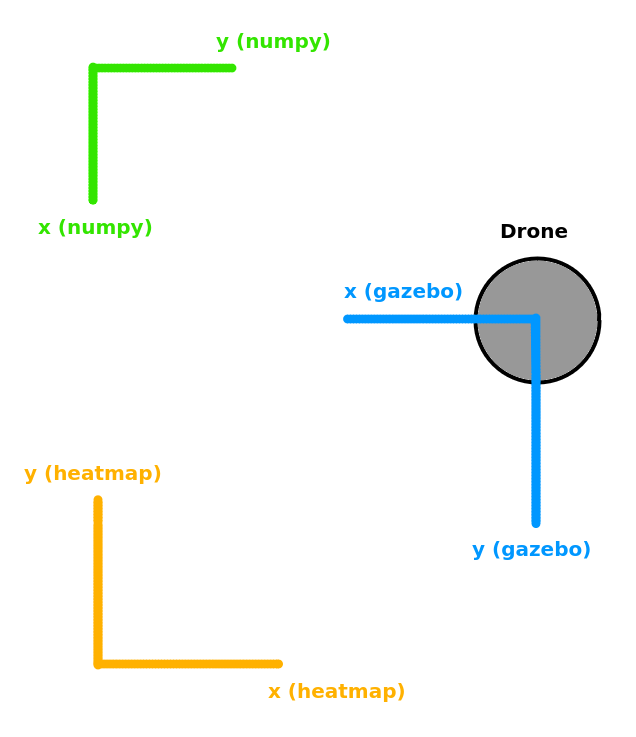
\includegraphics[height=10cm]{imagenes/cap4/8_reference_system.png}
    \end{center}
    \caption[Sistemas de referencia]{Sistemas de referencia}
    \label{fig:reference_sys}
\end{figure}

Por último y antes de entrar en los detalles de cada algoritmo, se deben cumplir una serie de premisas de cara a la simulación.\\ 

Estas son que, todos los movimientos realizados por el dron deben estar contenidos en el mapa de calor generado; además, la medida de la señal sólo podrá tomarse cuando el dron esté en el centro de la celda; los movimientos del dron deberán ser de centro en centro aunque esto abarque más celdas de distancia (problema resuelto y adaptado del teleoperador); y que la métrica de cada celda es de 1x1 metros.

\subsubsection{Algoritmo manual}
\label{subsec:alg-manual}

Es básicamente la primera aproximación, consiste en visitar todos los vecinos más cercanos y realizar el desplazamiento hacia las coordenadas del vecino con mayor señal medida.\\

La condición de parada analiza si las coordenadas objetivo de la iteración anterior, son las mismas que las coordenadas objetivo de la iteración actual, además, se debe cumplir que todos los vecinos colindantes tengan un valor de la señal menor.\\

En cuanto a los métodos que se usan, se encuentra el de verificar movimientos válidos y el de comprobar si ha llegado a la casilla final, mediante la verificación anterior (vecindad con menor señal).\\

\begin{figure} [H]
    \begin{center}
    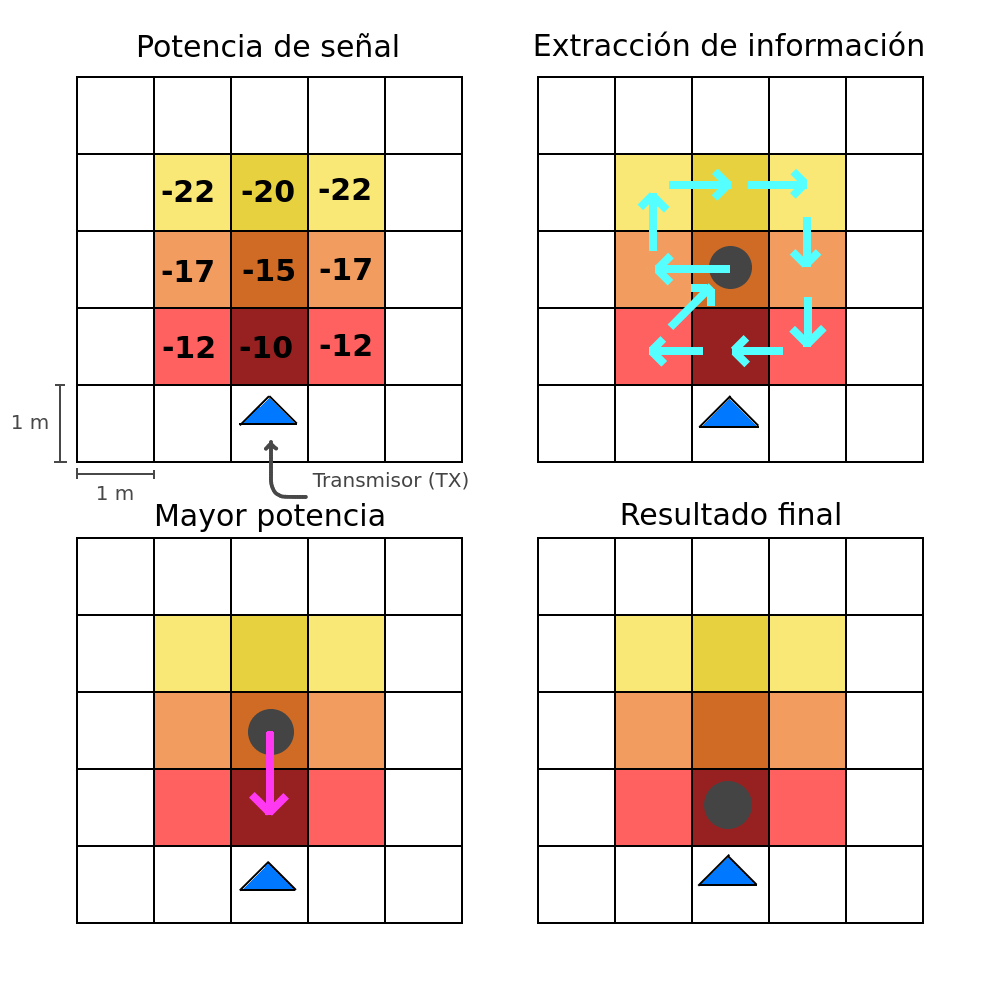
\includegraphics[height=10cm]{imagenes/cap4/9_algoritmo_manual.png}
    \end{center}
    \caption[Representación algoritmo manual]{Representación algoritmo manual}
    \label{fig:manual_algorithm}
\end{figure}

\subsubsection{Algoritmo manual (optimizado)}
\label{subsec:alg-manual-opt}

Tomando como referencia el algoritmo anterior, se han agregado ciertas mejoras y eficiencia. El principio es el mismo, se obtiene la información de los vecinos y se navega hacia el mejor candidato.\\

La diferencia radica en no revisitar vecinos cuya información se conozce. Para ello, se ha implementado un array que almacena hasta 18 coordenadas de vecinos visitados, de modo que solo se navega hacia coordenadas nuevas, y que por supuesto cumplan las condiciones del problema (no salirse del mapa de calor, moverse de centro a centro, entre otras).\\

La condición de parada es idéntica a la anterior, y los métodos usados también.\\

\begin{figure} [H]
    \begin{center}
    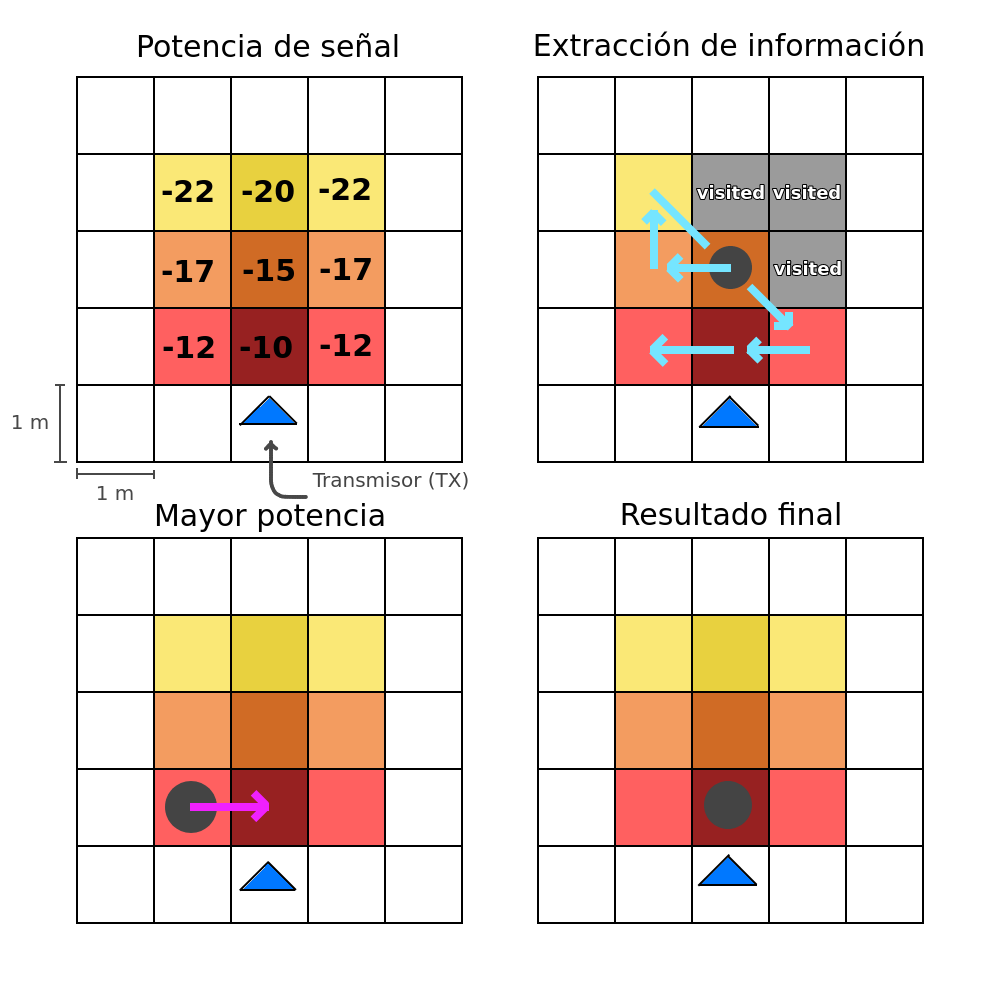
\includegraphics[height=10cm]{imagenes/cap4/10_algoritmo_optimizado.png}
    \end{center}
    \caption[Representación algoritmo manual optimizado]{Representación algoritmo manual optimizado}
    \label{fig:opt_algorithm}
\end{figure}

\subsubsection{Algoritmo Q-Learning}
\label{subsec:alg-q}

Por último, se ha planteado un algoritmo basado en técnicas de aprendizaje por refuerzo. Concretamente empleando Q-Learning, que tal y como comentamos al principio de la memoria, consiste en la obtención de una tabla Q, de estados y acciones, donde se asignan valores numéricos cada acción según su estado, de modo que la acción más favorable acaba teniendo mayor valor numérico que el resto.\\

En nuestro caso, los estados son las coordenadas del dron en términos del mapa de calor, y las acciones son los movimientos cardinales y diagonales, de una o más celdas de distancia.\\

Como todo algoritmo de esta naturaleza, se distinguen dos fases: la fase de entrenamiento, cuyo objetivo es rellenar de forma eficaz la tabla Q, y la fase de inferencia, donde se prueban los resultados obtenidos durante el entrenamiento.\\

Dentro del entrenamiento, podemos encontrar episodios, que en nuestro caso son las llegadas a la casilla final, o a casillas fuera del mapa definido (adicionalmente se añadió otra condición basada en el número de malas acciones consecutivas, pero de cara a extraer el máximo número de datos posibles para la tabla Q, esta condición no era adecuada, por ello se obvió); y las iteraciones, que se definen literalmente como la realización de una acción.\\

Además, para rellenar el contenido de la tabla, se han definido las pertinentes recompensas y penalizaciones basadas en la diferencia entre la medidas, antes y después de realizar una acción (agregando un pequeño multiplicador a las recompensas negativas), contemplando casos extra, como cuando el dron se sale del mapa, donde se establece una recompensa fija negativa, calculada en proporción al resto de recompensas. Posteriormente, se asignan los valores obtenidos en la tabla Q, haciendo uso de la ecuación de Bellman:
\begin{equation}
    Q(s, a) = (1 - \alpha) \cdot Q(s, a) + \alpha \cdot \left(r + \gamma \cdot \mathrm{max}_{a'} Q(s', a')\right)
\end{equation}
Cabe destacar que, durante el entrenamiento, se especifican una serie de parámetros que han sido ajustados a través de la experimentación, estos son: el número de episodios totales, que repercute directamente en la \emph{fase de exploración} (detallado a continuación); el parámetro $\alpha$, o la tasa de aprendizaje, que afecta a la convergencia de las soluciones durante el aprendizaje; el parámetro $\gamma$, o factor de descuento, que alude a la importancia de las acciones futuras con respecto a las inmediatas; y por último los valores de epsilon ($\epsilon$), que determinan si la acción tomada será aleatoria o extraida de la tabla, esto está directamente asociado a la \emph{fase de exploración}, donde se prioriza la aleatoreidad con el fin de enriquecer con información la tabla Q.\\

En nuestro caso, esta fase ocupa un 20\% del número de episodios, de forma lineal, es decir, que cada vez la prioridad se va decantando más del lado de la tabla y no de la aleatoreidad (durante el entrenamiento siempre se mantiene cierta posibilidad de tomar una acción arbitraria, para seguir actualizando los datos).\\

Para poder entrenar de forma eficiente, se han establecido distintos puntos de entrenamiento repartidos de forma uniforme por el mapa, tal y como se mencionará en la sección de métricas.\\

Los métodos usados para Q-Learning, se basan en las funcionalidades necesarias para desempeñar todo el proceso definido anteriormente, véase la generación de estados y acciones para la tabla, la extracción de índices dentro de la misma, el tratamiento del parámetro $\epsilon$, la obtención de coordenadas válidas, entre otros\footnote[3]{Todos los métodos están explicados dentro del código \url{https://github.com/RoboticsLabURJC/2022-tfg-cristian-sanchez/blob/main/src/teleop/scripts/algorithms.py}}.\\

\begin{figure} [H]
    \begin{center}
    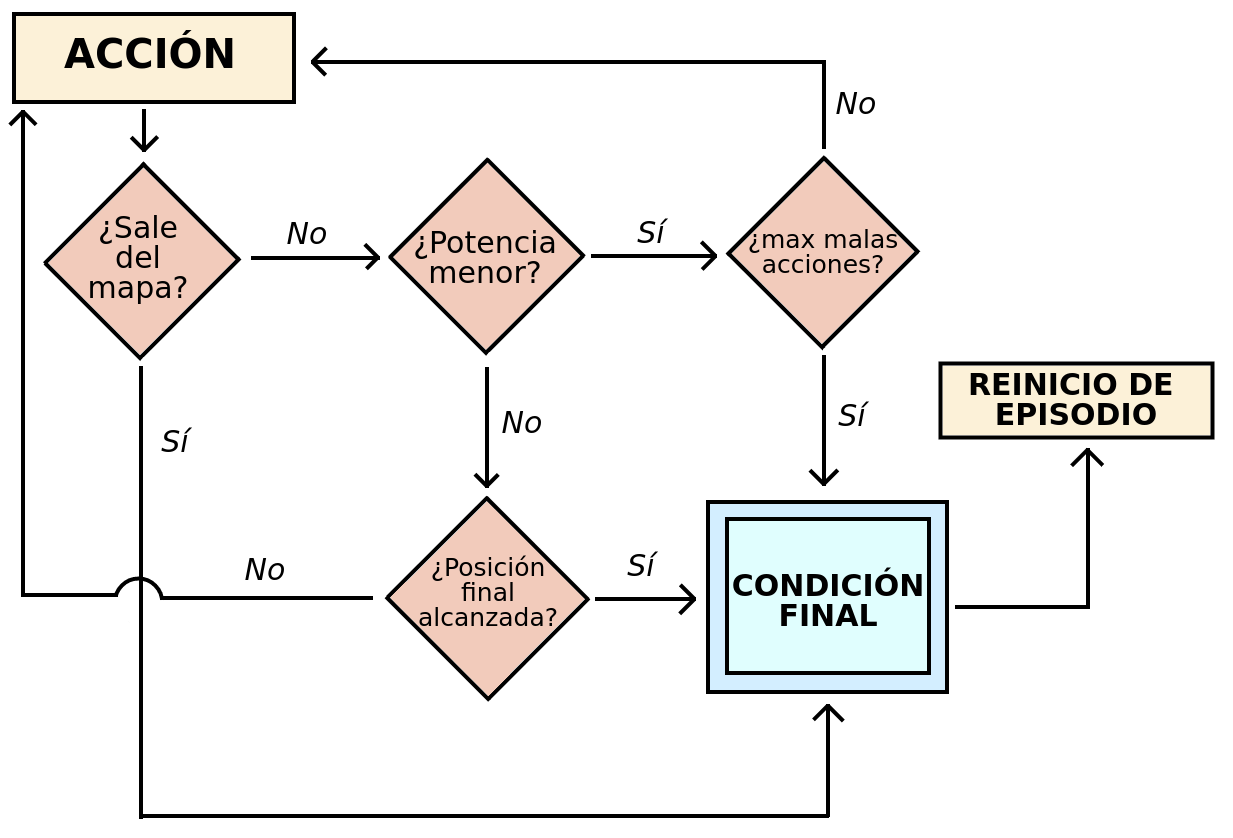
\includegraphics[height=10cm]{imagenes/cap4/11_diagrama_training.png}
    \end{center}
    \caption[Esquema episodio fase de entrenamiento]{Esquema episodio fase de entrenamiento}
    \label{fig:training_phase}
\end{figure}

Cabe destacar que, si la acción tomada lleva al dron hacia una condición de final, este finaliza automáticamente el episodio, viajando hacia una nueva posición de entrenamiento y actualizando ciertos parámetros, como es el caso  del parámetro $\epsilon$. La condición de final se aplica siempre tras actualizar los valores intrínsecos en la iteración.\\

Por último, en la \emph{fase de inferencia}, el dron analiza su estado (o sus coordenadas dentro del mapa de calor), y observa la mejor acción disponible dentro de la tabla Q ya rellena. Esto lo realiza hasta que detecta la condición de parada, que se cumple cuando la medida anterior de señal es mayor que la actual y todos los vecinos adyacentes a la mayor de las medidas, poseen señal inferior. Para hacer un correcto análisis, se parte siempre de coordenadas distintas a las que se usaron para entrenar y rellenar la tabla Q.

\subsection{Experimentos y resultados}
\label{subsec:experimentos_sf}

\subsubsection{Tipos de gráficos}
\label{subsubsec:graficos}

Antes de entrar en las pruebas realizadas, es conveniente introducir el tipo de gráficos que han sido usados.\\

En primer lugar se encuentra el mapa de puntos. Aquí se muestran las posiciones en el mapa de calor donde el dron entrena, infiere (o desde donde empieza a moverse en los algoritmos), además de la posición de la señal y propios los límites del mapa.\\

\begin{figure} [H]
    \begin{center}
    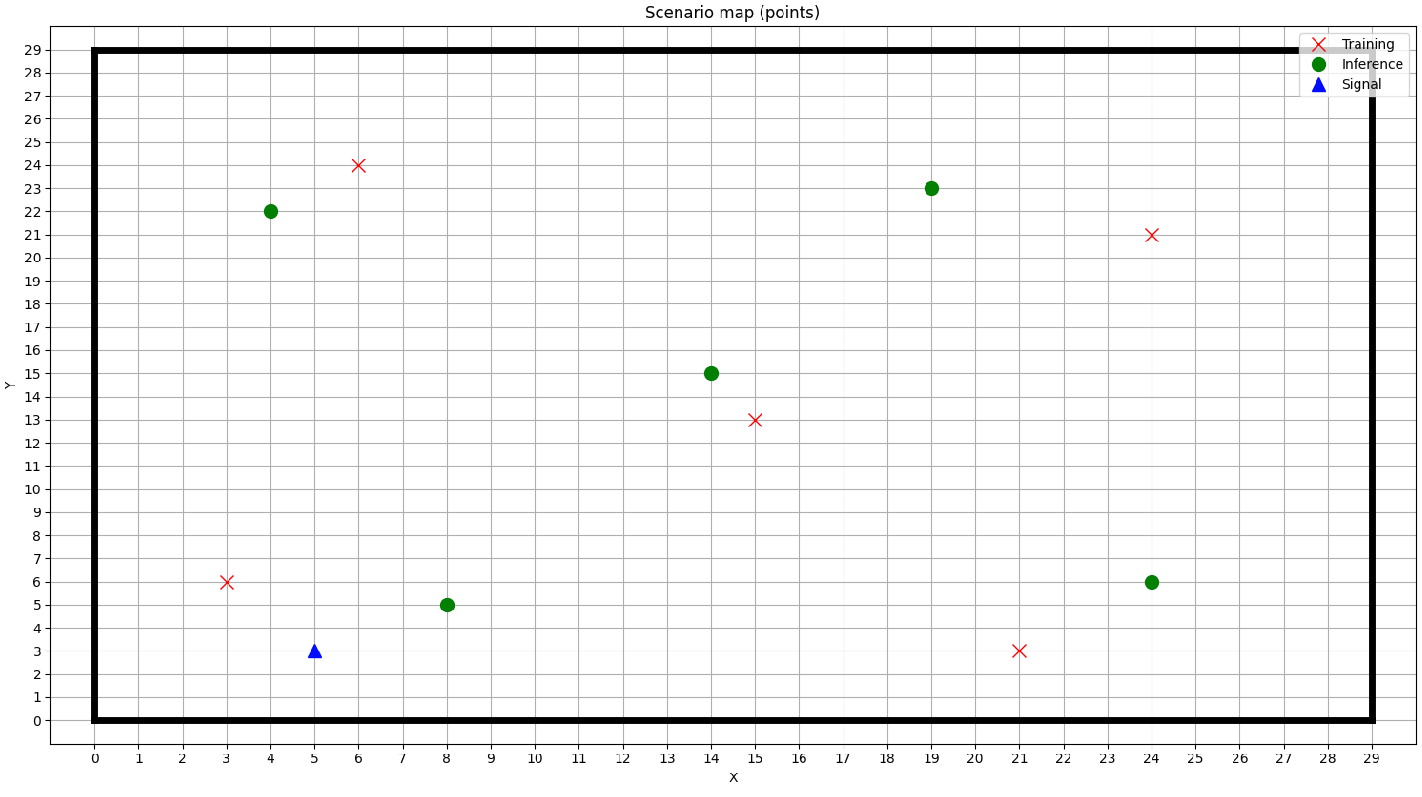
\includegraphics[height=7cm]{imagenes/cap4/12_puntos_30_esquina.png}
    \end{center}
    \caption[Mapa de puntos 30x30 con la señal en la esquina]{Mapa de puntos 30x30 con la señal en la esquina}
    \label{fig:30_points}
\end{figure}

El siguiente gráfico representa el camino seguido por el dron al aplicar cada algoritmo para unas mismas coordenadas.\\

\begin{figure} [H]
    \begin{center}
    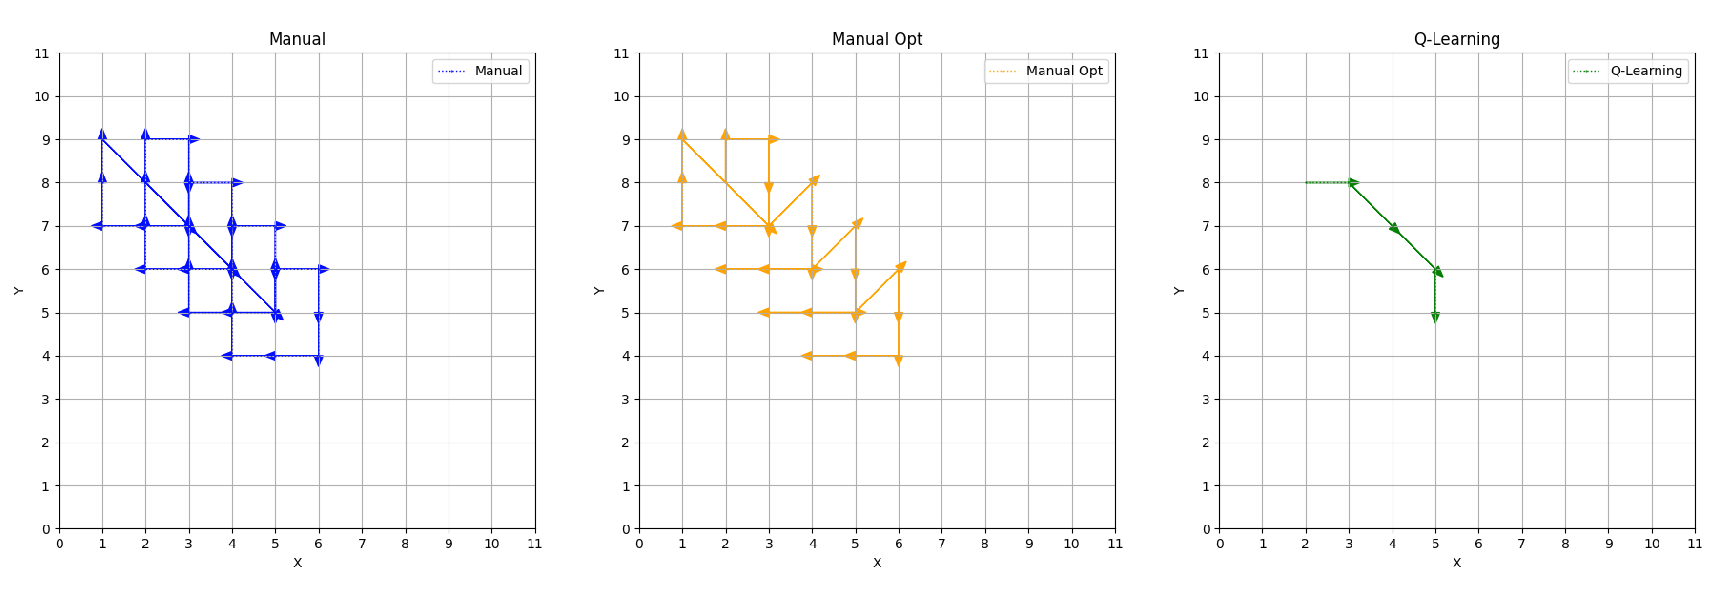
\includegraphics[height=5cm]{imagenes/cap4/13_trayectorias_12.png}
    \end{center}
    \caption[Trayectorias seguidas en mapa 12x12 con señal en el centro]{Trayectorias seguidas en mapa 12x12 con señal en el centro}
    \label{fig:12_traj}
\end{figure}

A continuación se presenta uno de los gráficos más relevantes, en este caso, un gráfico triple que nos permite conocer en detalle como ha ido el entrenamiento. En concreto, representa tres métricas: el valor de epsilon ($\epsilon$), en el que se distingue la fase de exploración; la recompensa acumulada, que nos permite analizar la convergencia del entrenamiento; y el número de iteraciones, donde se observa que conforme el algoritmo aprende, el número se reduce. Todo ello con respecto a cada episodio.\\

\begin{figure} [H]
    \begin{center}
    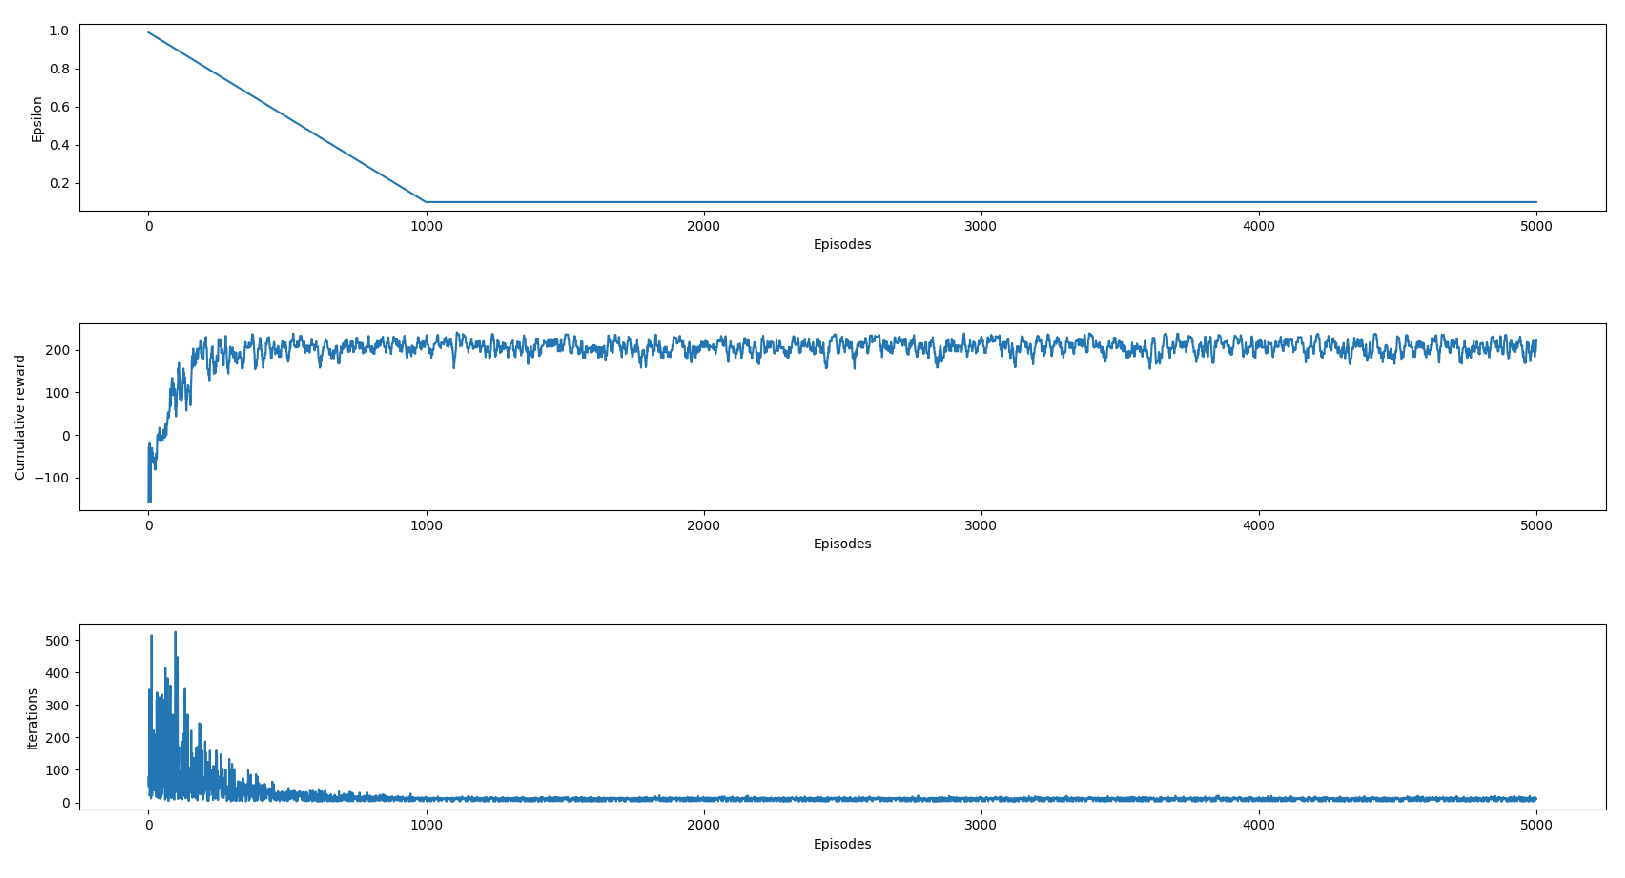
\includegraphics[height=8cm]{imagenes/cap4/14_training_graph.png}
    \end{center}
    \caption[Gráfico de entrenamiento]{Gráfico de entrenamiento}
    \label{fig:training_graph}
\end{figure}

Por último, se muestran los gráficos comparativos que nos dan un aproximado del rendimiento de cada algoritmo. En este caso, también se analizan tres cosas: el tiempo medio en segundos que tarda el dron desde que despega hasta que vuelve a su posición de despegue; el número medio de iteraciones empleadas para alcanzar la señal; y el número medio de movimientos hacía coordenadas donde la señal es menor y no mayor\footnote[4]{Los datos arrojados han sido guardados en formato \emph{csv}.}.\\

\begin{figure} [H]
    \begin{center}
    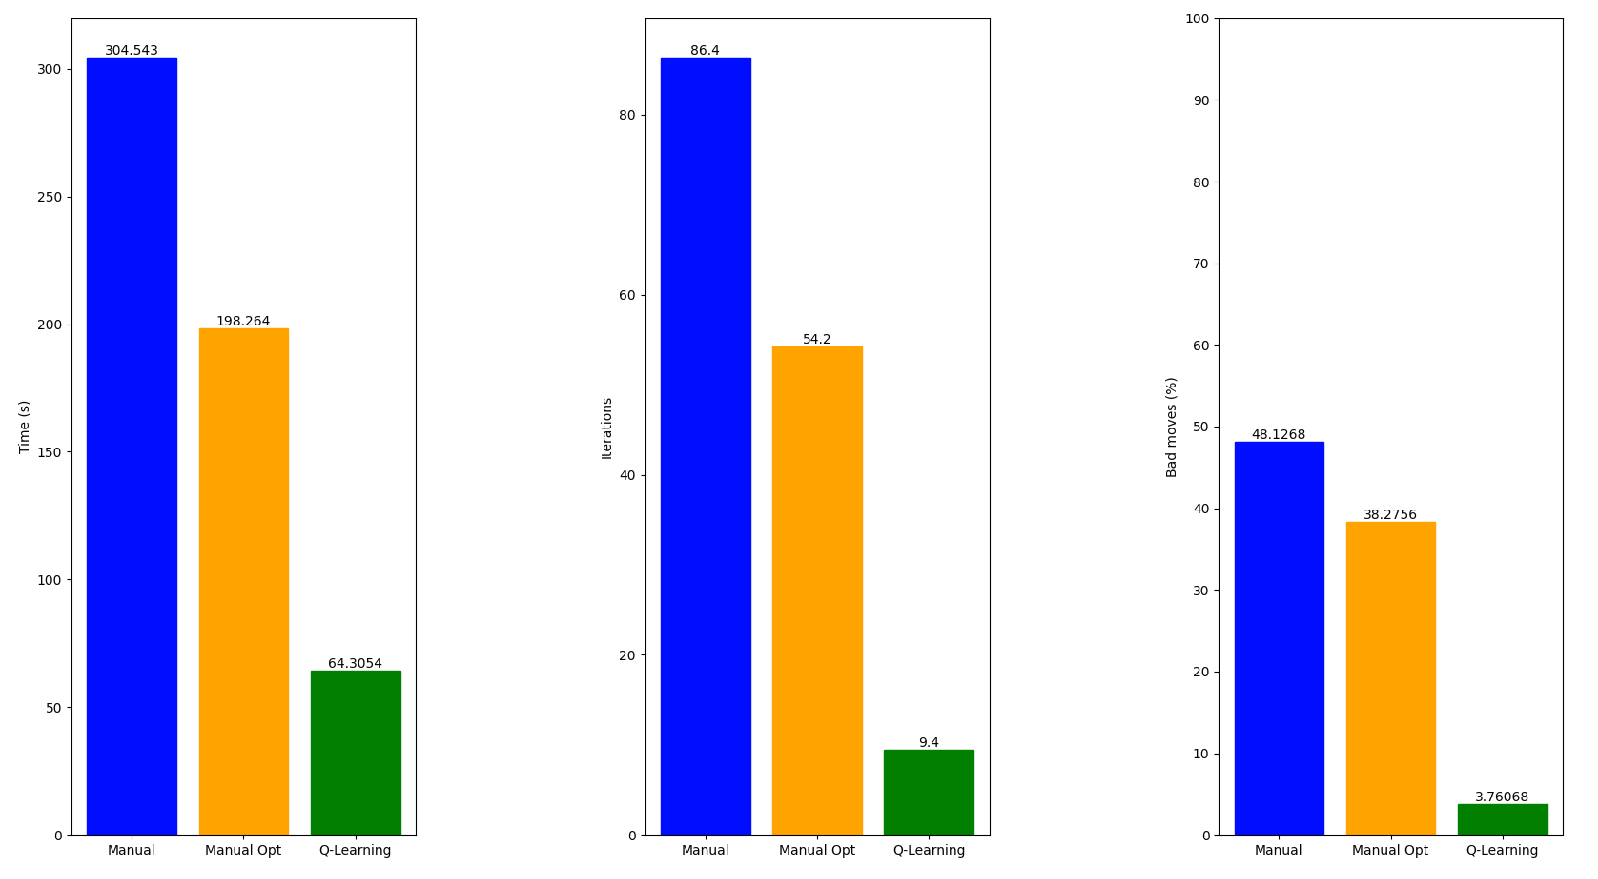
\includegraphics[height=8cm]{imagenes/cap4/15_avg_graphs.png}
    \end{center}
    \caption[Gráficos comparativos]{Gráficos comparativos}
    \label{fig:compare_graph}
\end{figure}

\subsubsection{Experimentos realizados}
\label{subsubsec:experimentos}

En cuanto a las pruebas realizadas propiamente dichas, y a excepción del último caso, los parámetros de la señal siempre son los valores por defecto establecidos en la clase, donde sólo varía el tamaño del mapa, que se va modificando según el experimento. Además, cabe destacar que la señal se toma como un punto estático dentro del mapa de calor y con respecto al dron, distinguiendo la posición centrada y la posición cercana a una esquina, que también dependen del experimento.\\

\begin{figure} [H]
    \begin{center}
    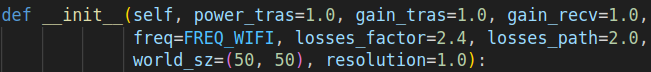
\includegraphics[height=1cm]{imagenes/cap4/16_default_values.png}
    \end{center}
    \caption[Características de la señal por defecto]{Características de la señal por defecto}
    \label{fig:compare_graph}
\end{figure}

Primero se ha probado sobre un escenario de tamaño 12x12 metros, con las dos posiciones de señal mencionadas:\\

Para la señal cerca del centro, situada en las coordenadas (5, 5) del \emph{``heatmap''}, se puede ver el siguiente mapa para los puntos de entrenamiento e inferencia:\\

\begin{figure} [H]
    \begin{center}
    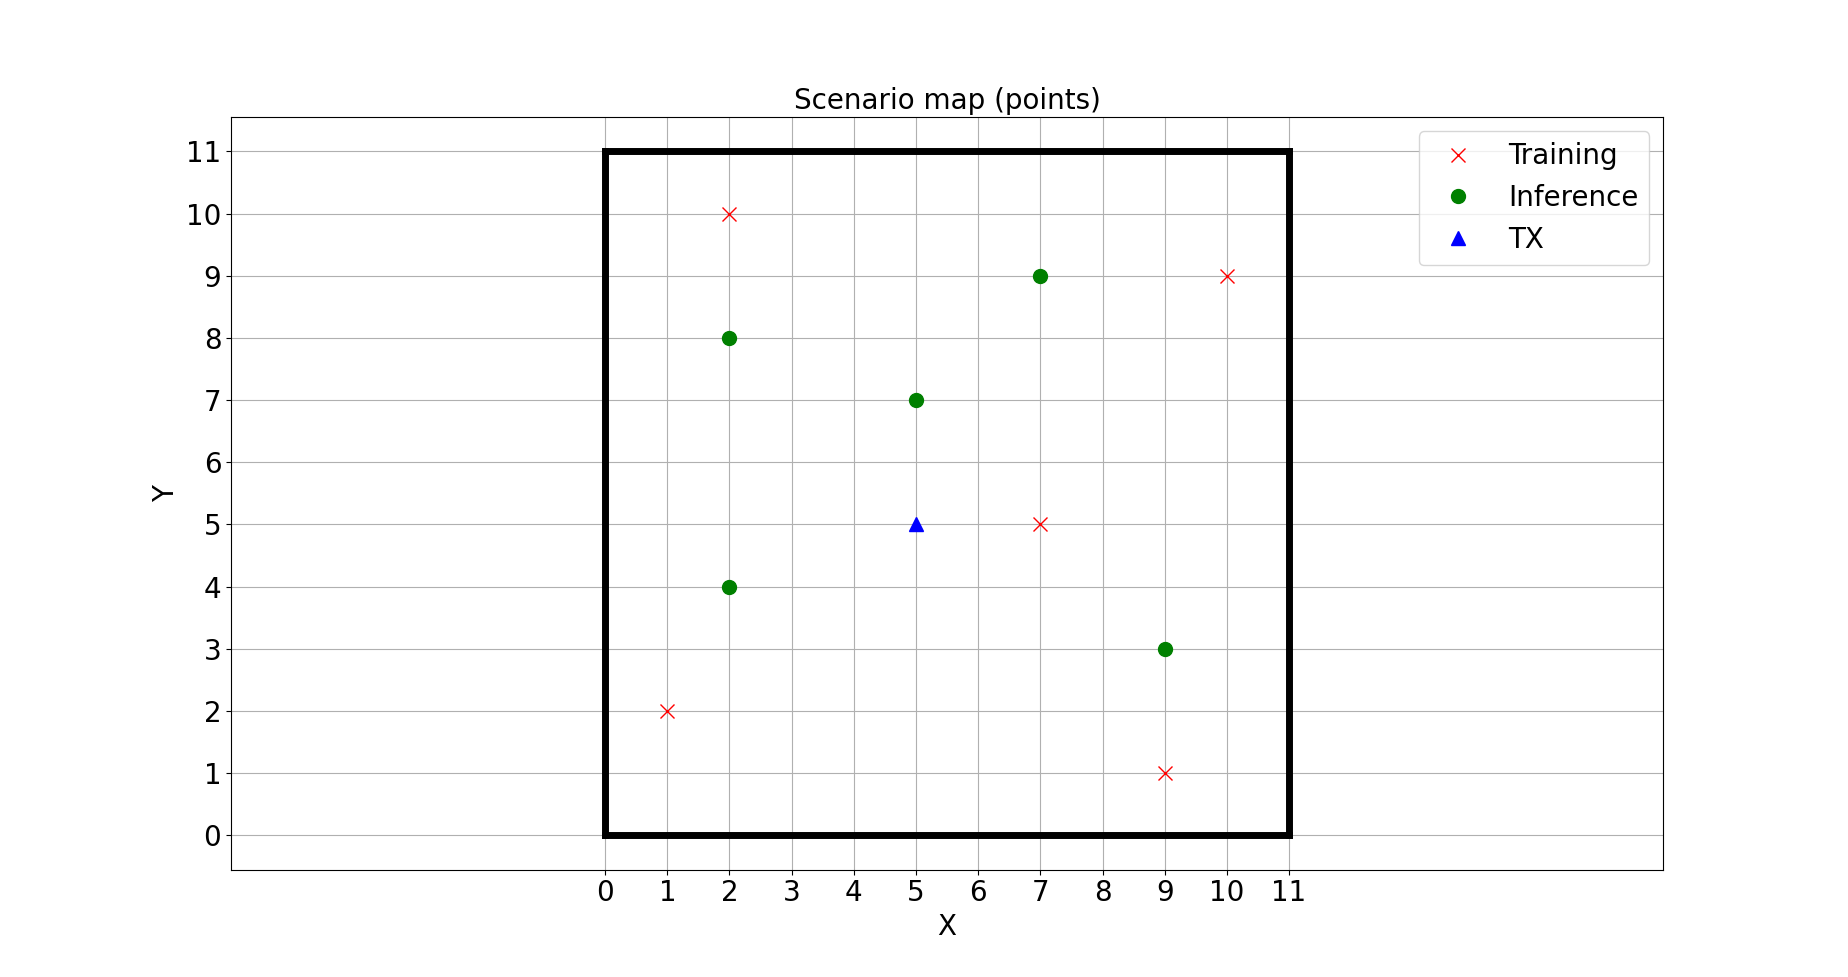
\includegraphics[height=8cm]{imagenes/cap4/17_mapa_p_centro_12.png}
    \end{center}
    \caption[Mapa de puntos (12x12), señal centrada]{Mapa de puntos (12x12), señal centrada}
    \label{fig:map_p_center_12}
\end{figure}

Los resultados obtenidos arrojan que el algoritmo más eficiente es el de Q-Learning, ya que tarda menos tiempo, realiza menos iteraciones hasta llegar a la meta y tiene un porcentaje inferior de malas acciones, tal y como se puede ver a continuación:\\

\begin{figure} [H]
    \begin{center}
    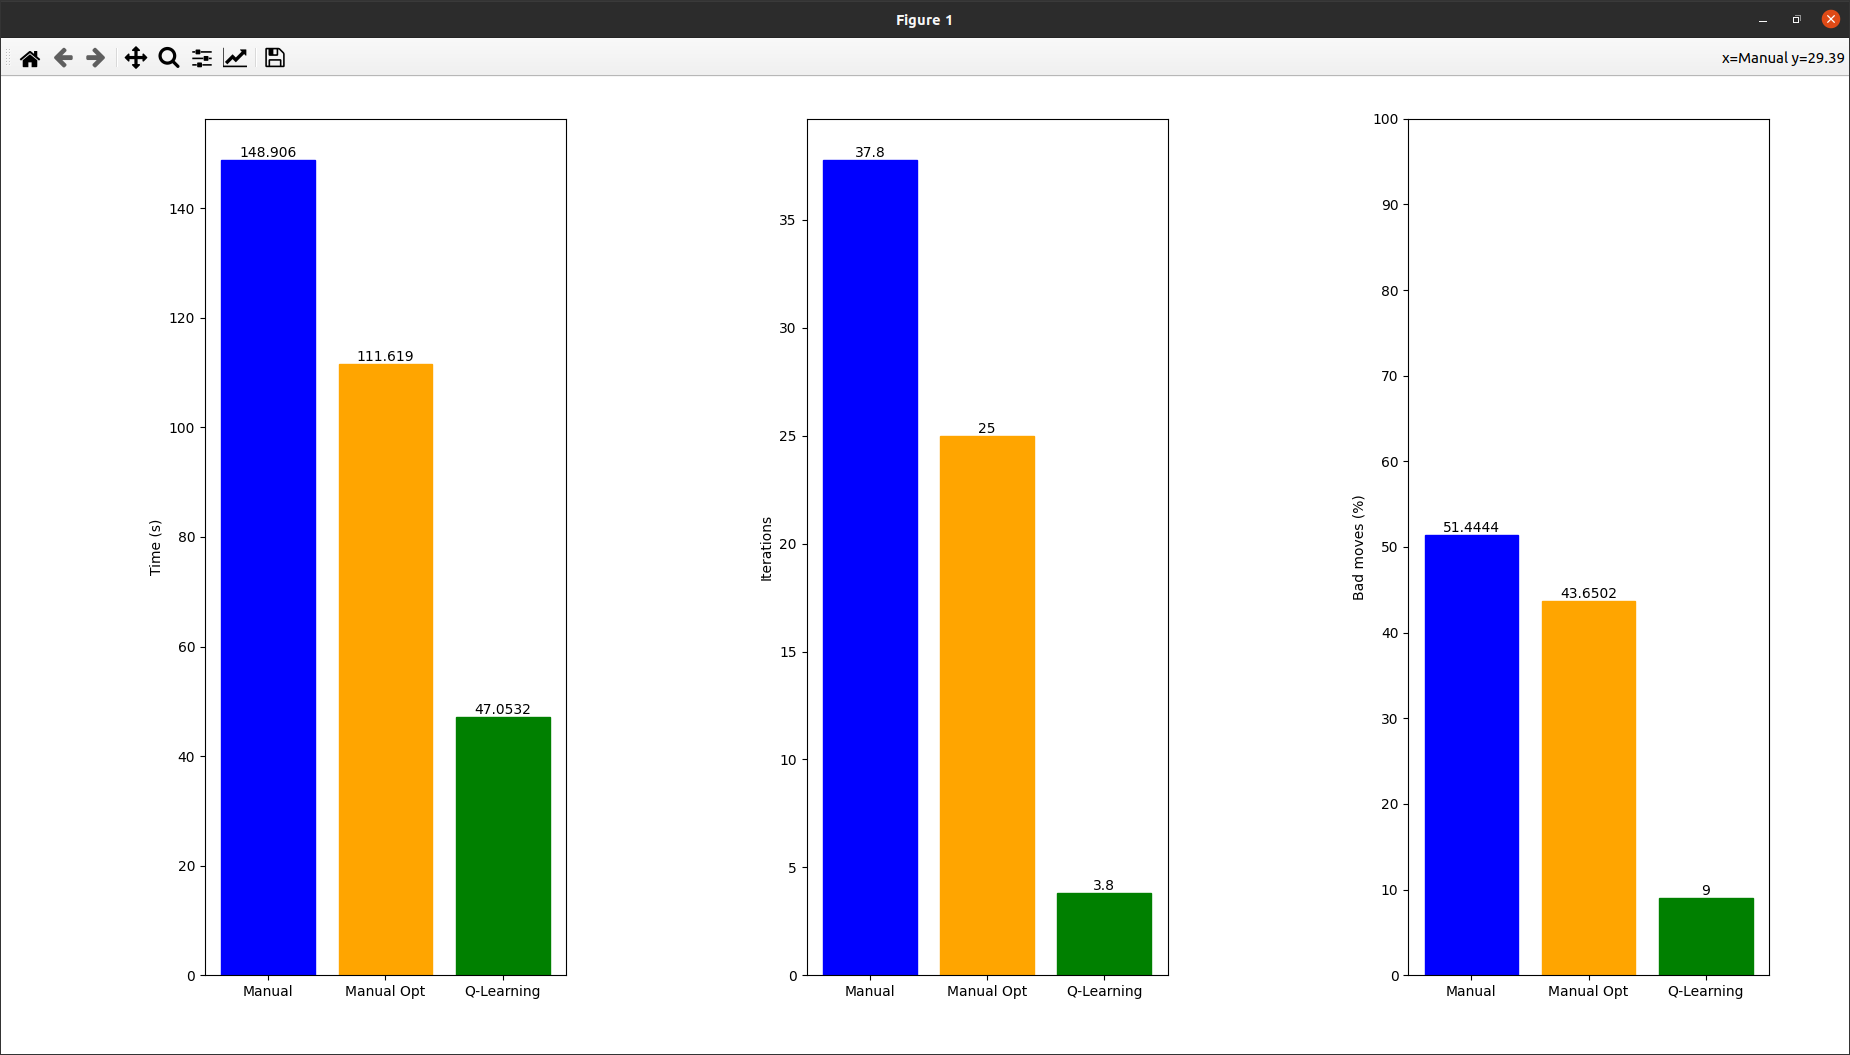
\includegraphics[height=8cm]{imagenes/cap4/18_comp_centro_12.png}
    \end{center}
    \caption[Comparativas (12x12), señal centrada]{Comparativas (12x12), señal centrada}
    \label{fig:comp_center_12}
\end{figure}

En el caso de la señal cerca de la esquina, la señal se sitúa en (3, 1) con respecto a las coordenadas del \emph{``heatmap''}, siendo su mapa de puntos el siguiente:

\begin{figure} [H]
    \begin{center}
    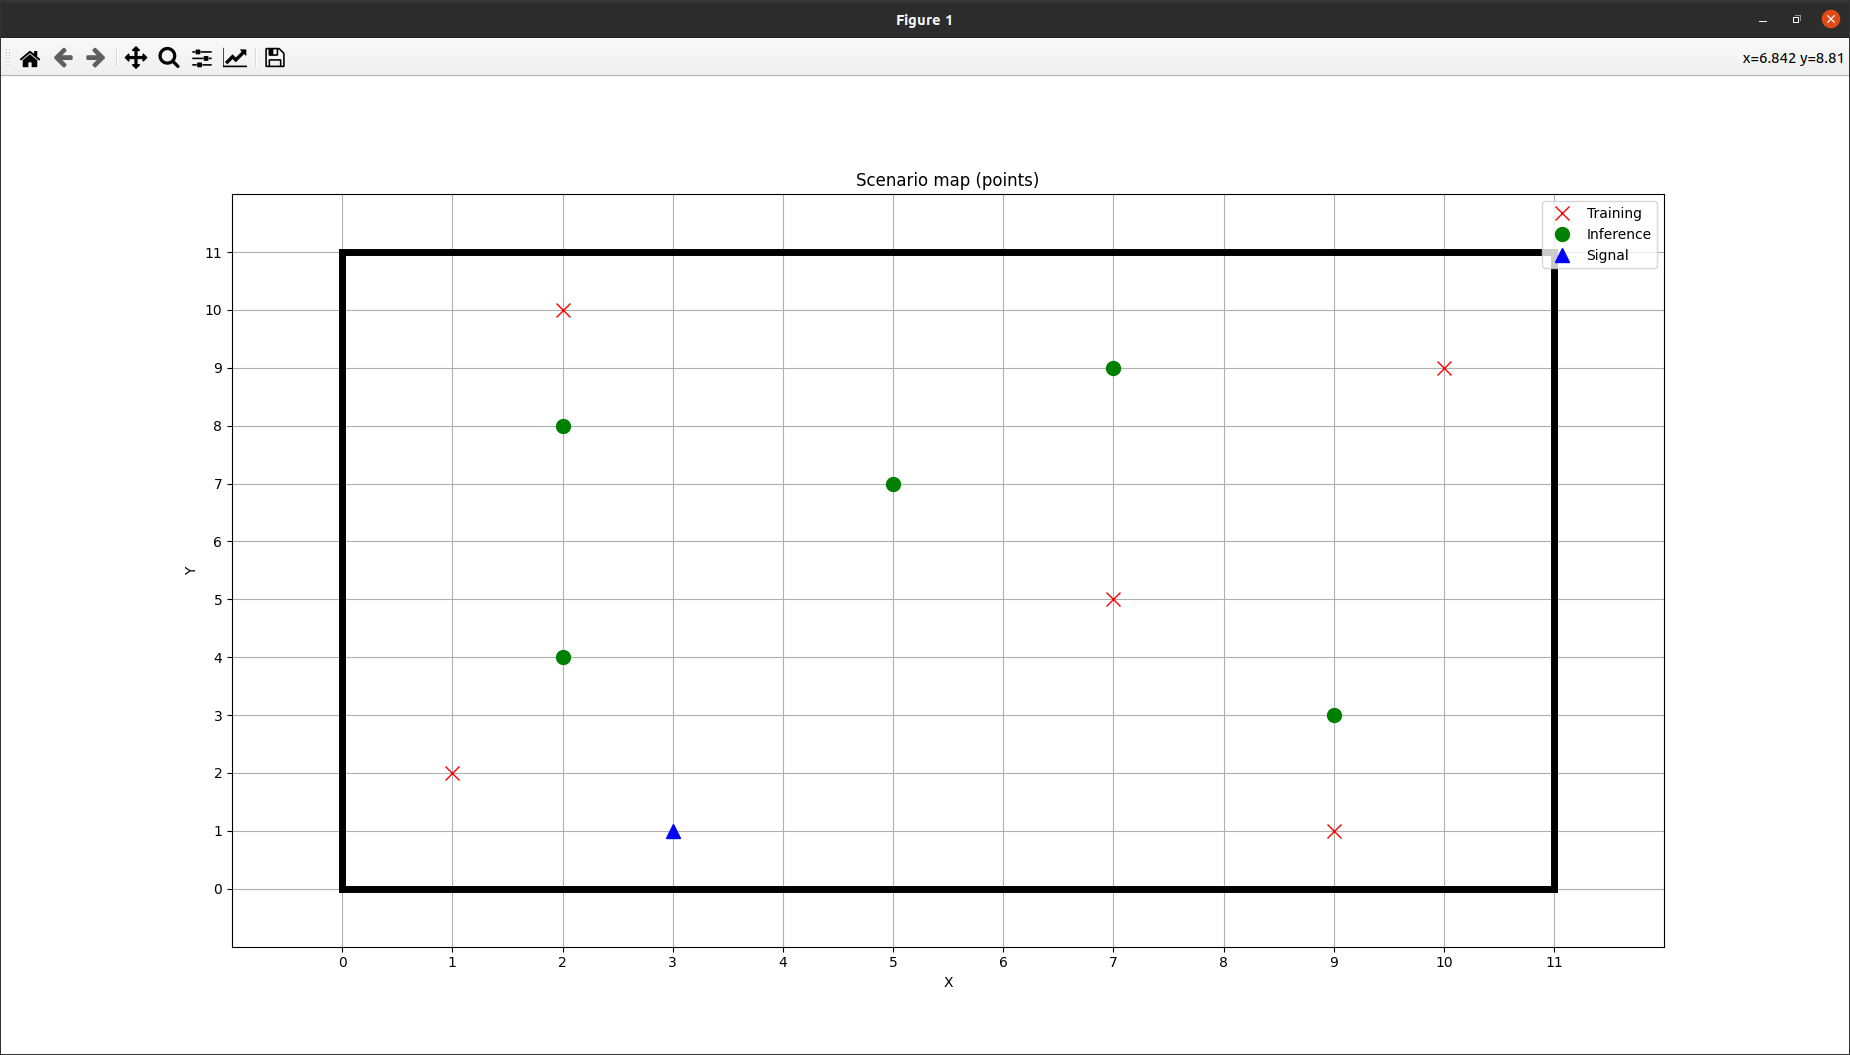
\includegraphics[height=8cm]{imagenes/cap4/19_mapa_p_esq_12.png}
    \end{center}
    \caption[Mapa de puntos (12x12), señal en la esquina]{Mapa de puntos (12x12), señal en la esquina}
    \label{fig:map_p_esq_12}
\end{figure}

En este caso, se obtiene la misma conclusión que en el escenario anterior, tal y como se ve a continuación:\\

\begin{figure} [H]
    \begin{center}
    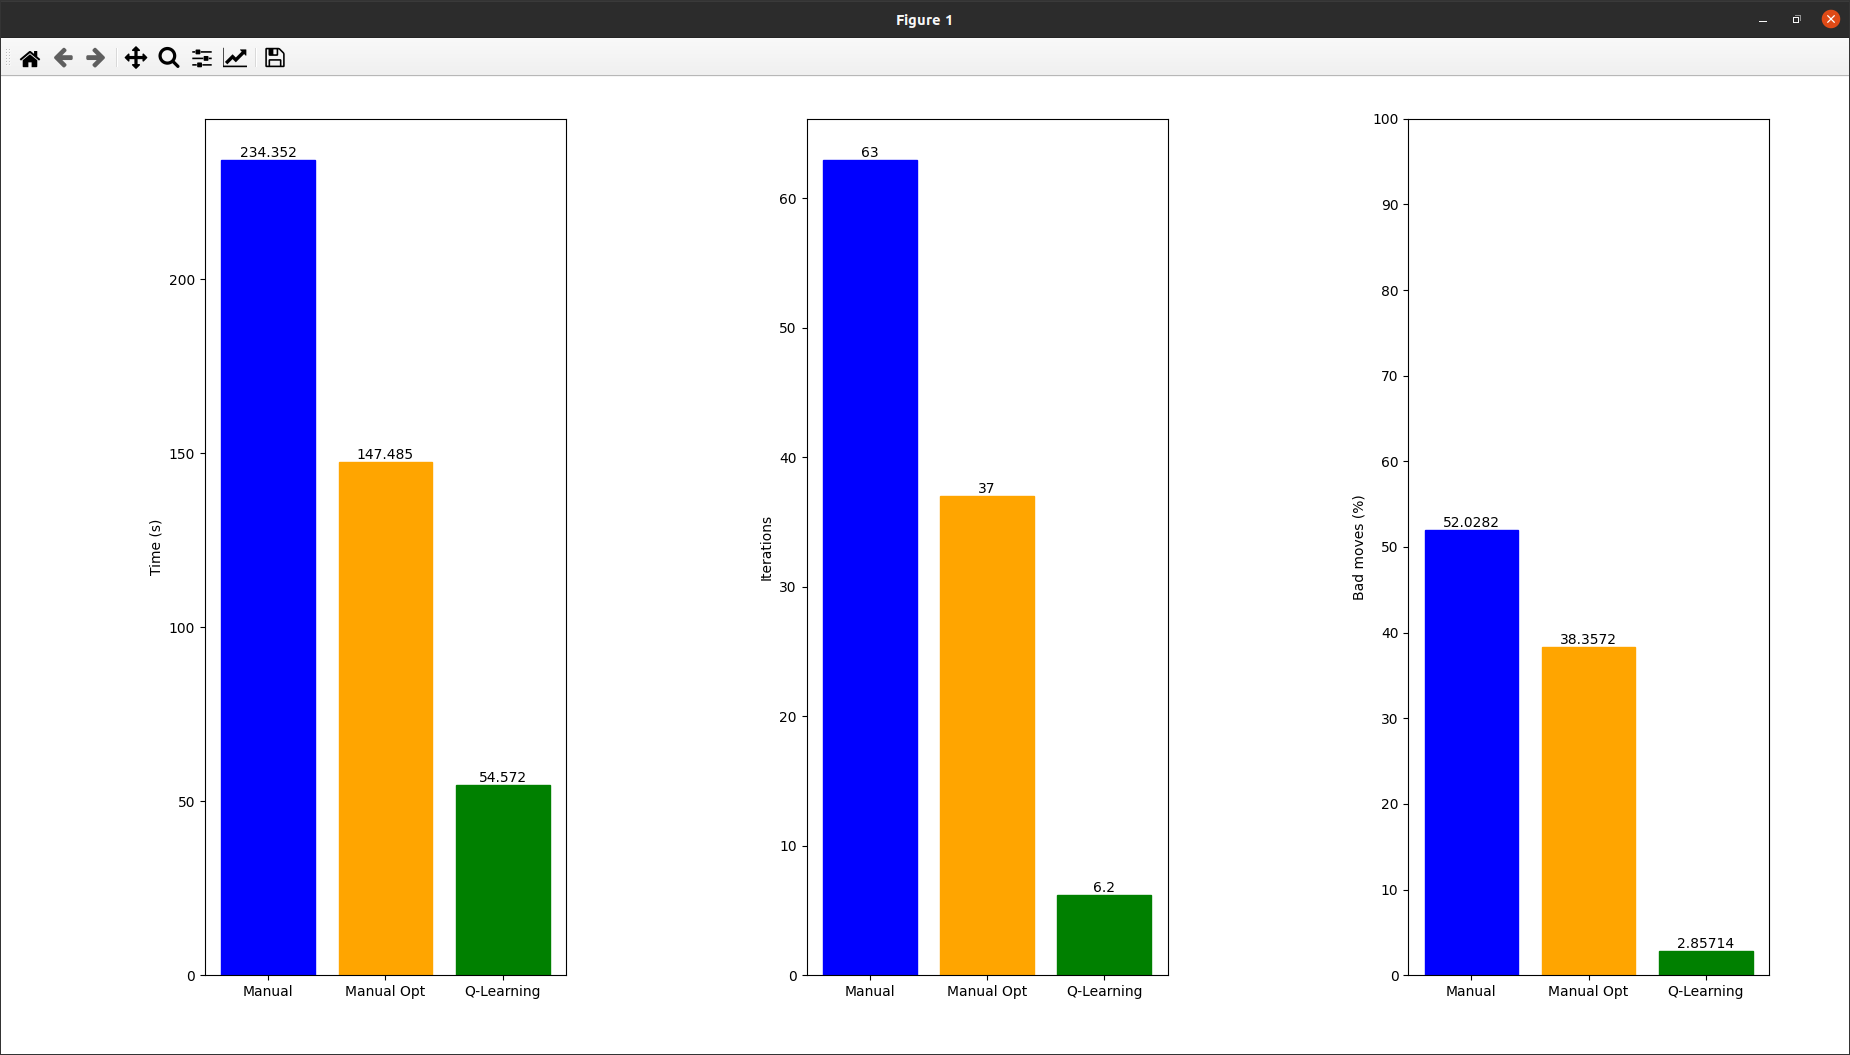
\includegraphics[height=8cm]{imagenes/cap4/20_comp_esq_12.png}
    \end{center}
    \caption[Comparativas (12x12), señal en la esquina]{Comparativas (12x12), señal en la esquina}
    \label{fig:comp_esq_12}
\end{figure}

En segundo lugar, se incrementa el tamaño del mapa hasta 30x30 metros.\\

Nuevamente, para la señal cerca del centro situada en este caso en las coordenadas (12, 12), tenemos:

\begin{figure} [H]
    \begin{center}
    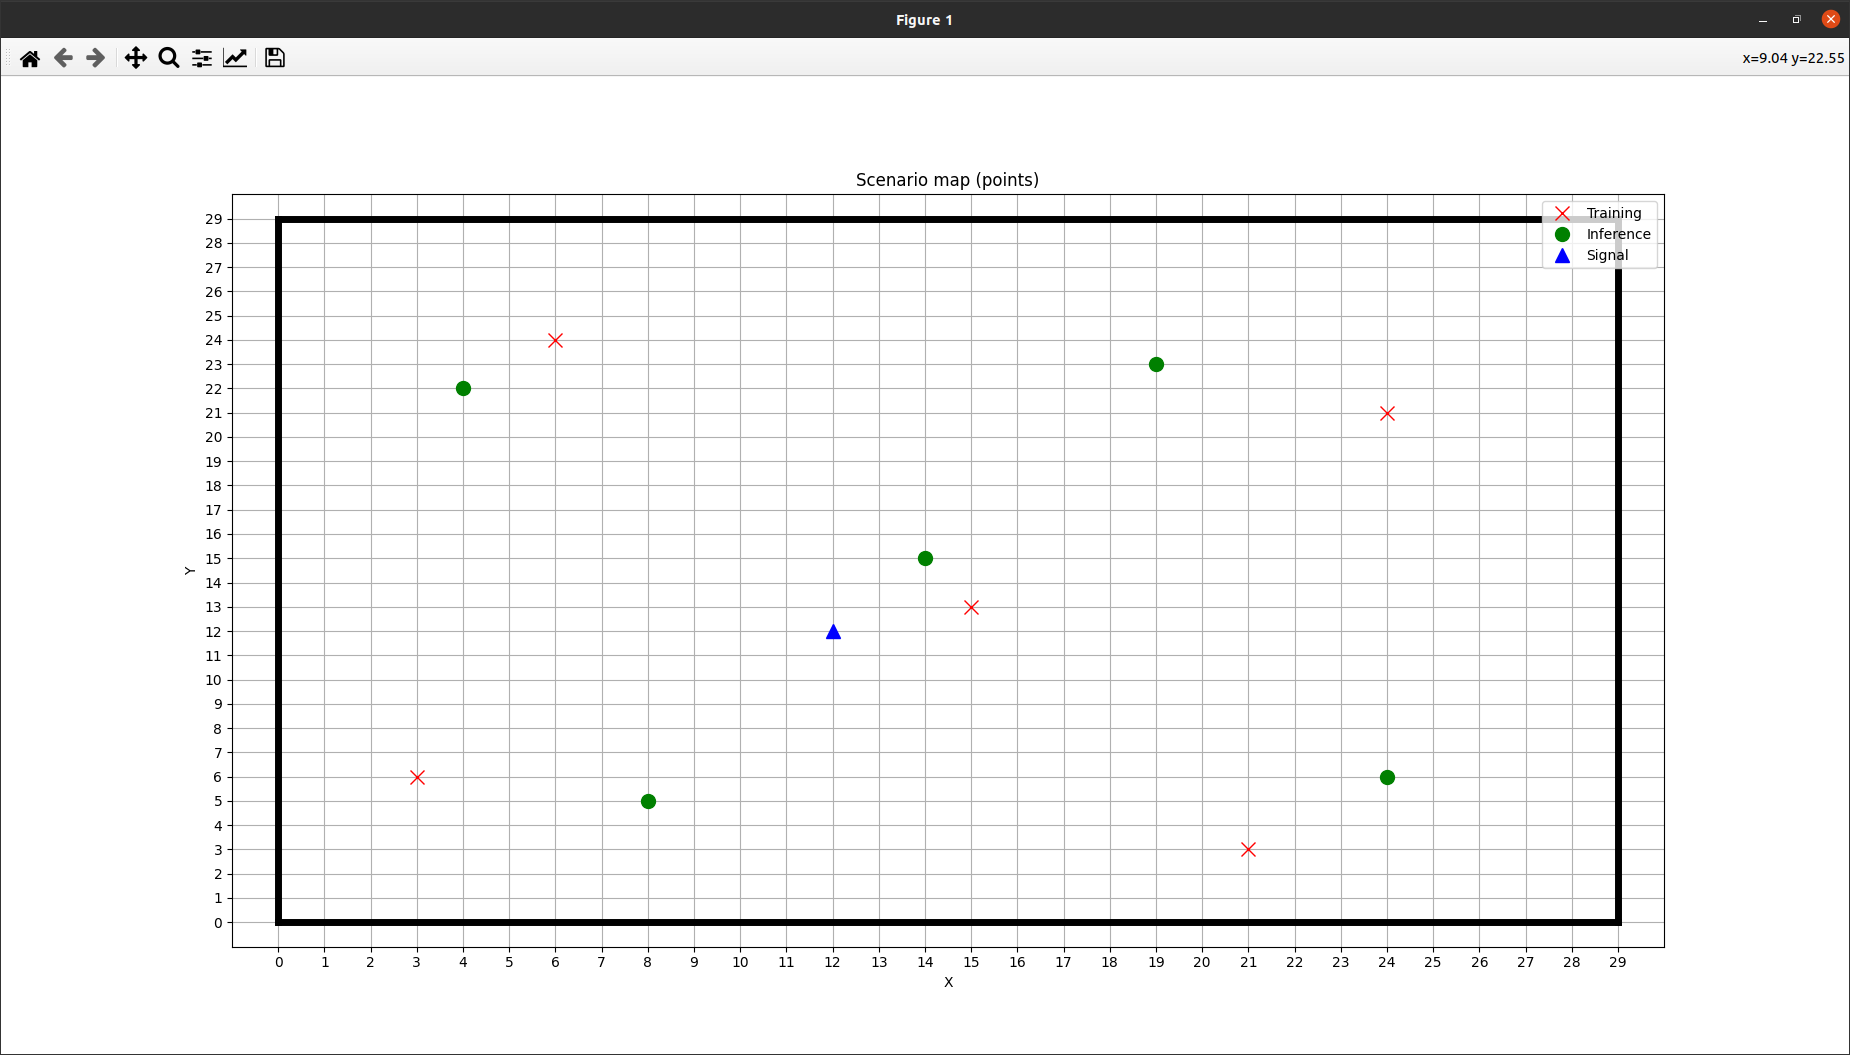
\includegraphics[height=8cm]{imagenes/cap4/21_mapa_p_centro_30.png}
    \end{center}
    \caption[Mapa de puntos (30x30), señal centrada]{Mapa de puntos (30x30), señal centrada}
    \label{fig:map_p_center_30}
\end{figure}

En cuanto a los resultados, se concluye que el algoritmo de Q-Learning vuelve a ser la mejor opción, aunque se vea un incremento temporal y de iteraciones por el aumento del tamaño del mapa, sigue siendo superior en todo al resto:\\

\begin{figure} [H]
    \begin{center}
    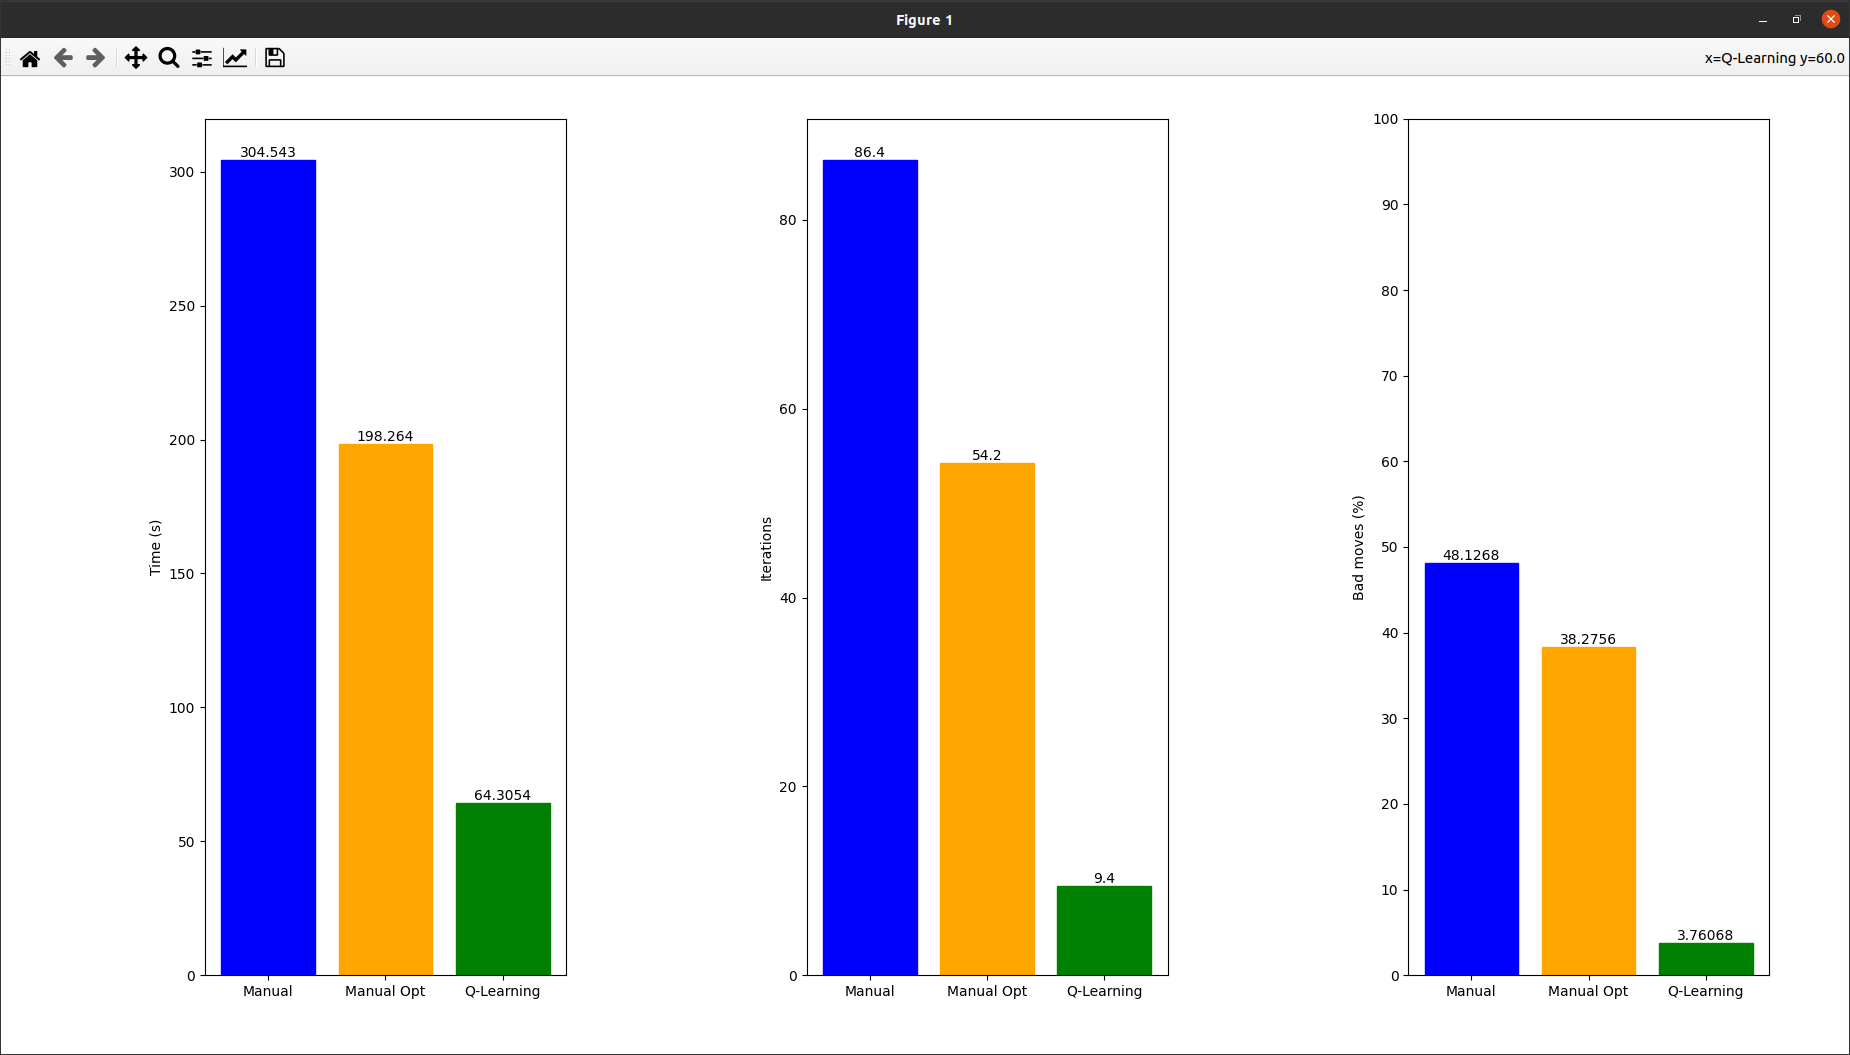
\includegraphics[height=8cm]{imagenes/cap4/22_comp_centro_30.png}
    \end{center}
    \caption[Comparativas (30x30), señal centrada]{Comparativas (30x30), señal centrada}
    \label{fig:comp_center_30}
\end{figure}

Continuando con la señal cerca de la esquina, que en este caso se encuentra en las coordenadas (5, 3), y donde su mapa de puntos es:\\

\begin{figure} [H]
    \begin{center}
    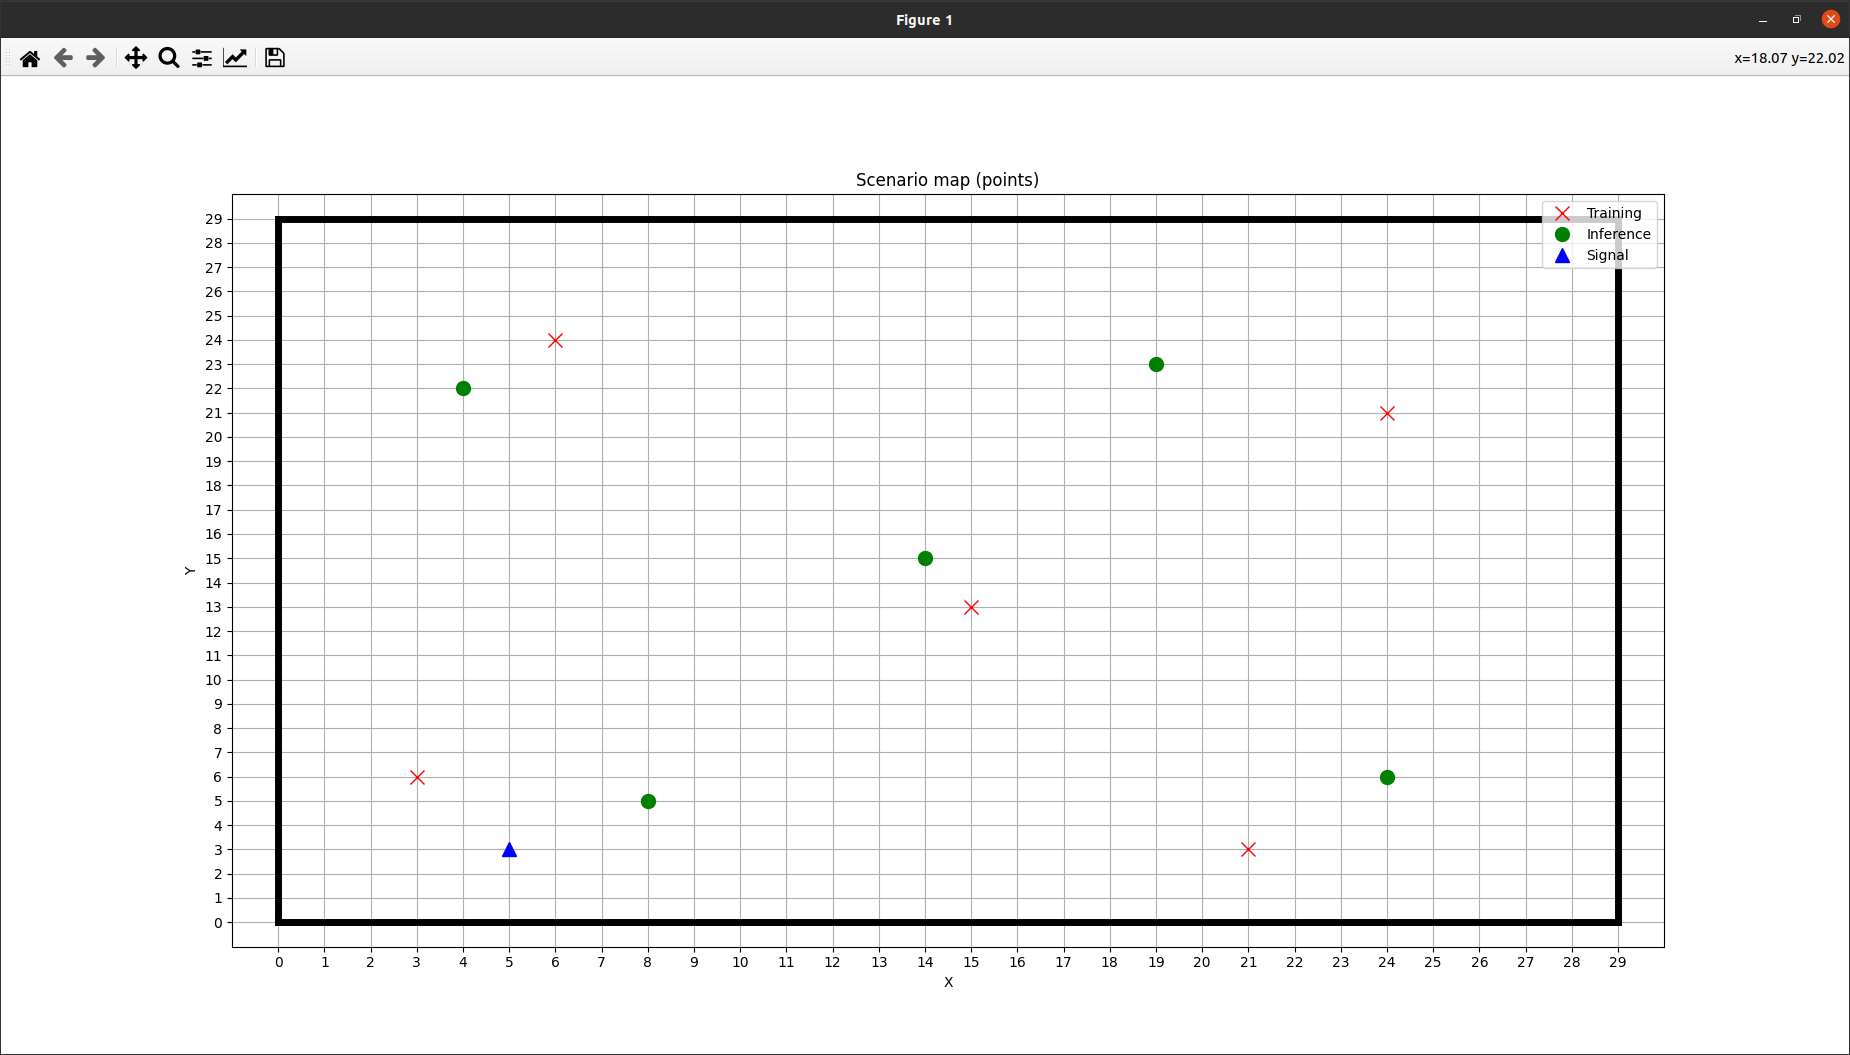
\includegraphics[height=8cm]{imagenes/cap4/23_mapa_p_esq_30.png}
    \end{center}
    \caption[Mapa de puntos (30x30), señal en la esquina]{Mapa de puntos (30x30), señal en la esquina}
    \label{fig:map_p_esq_30}
\end{figure}

Vemos que el resultado de aprendizaje por refuerzo es claramente nuevamente mejor que el resto:\\

\begin{figure} [H]
    \begin{center}
    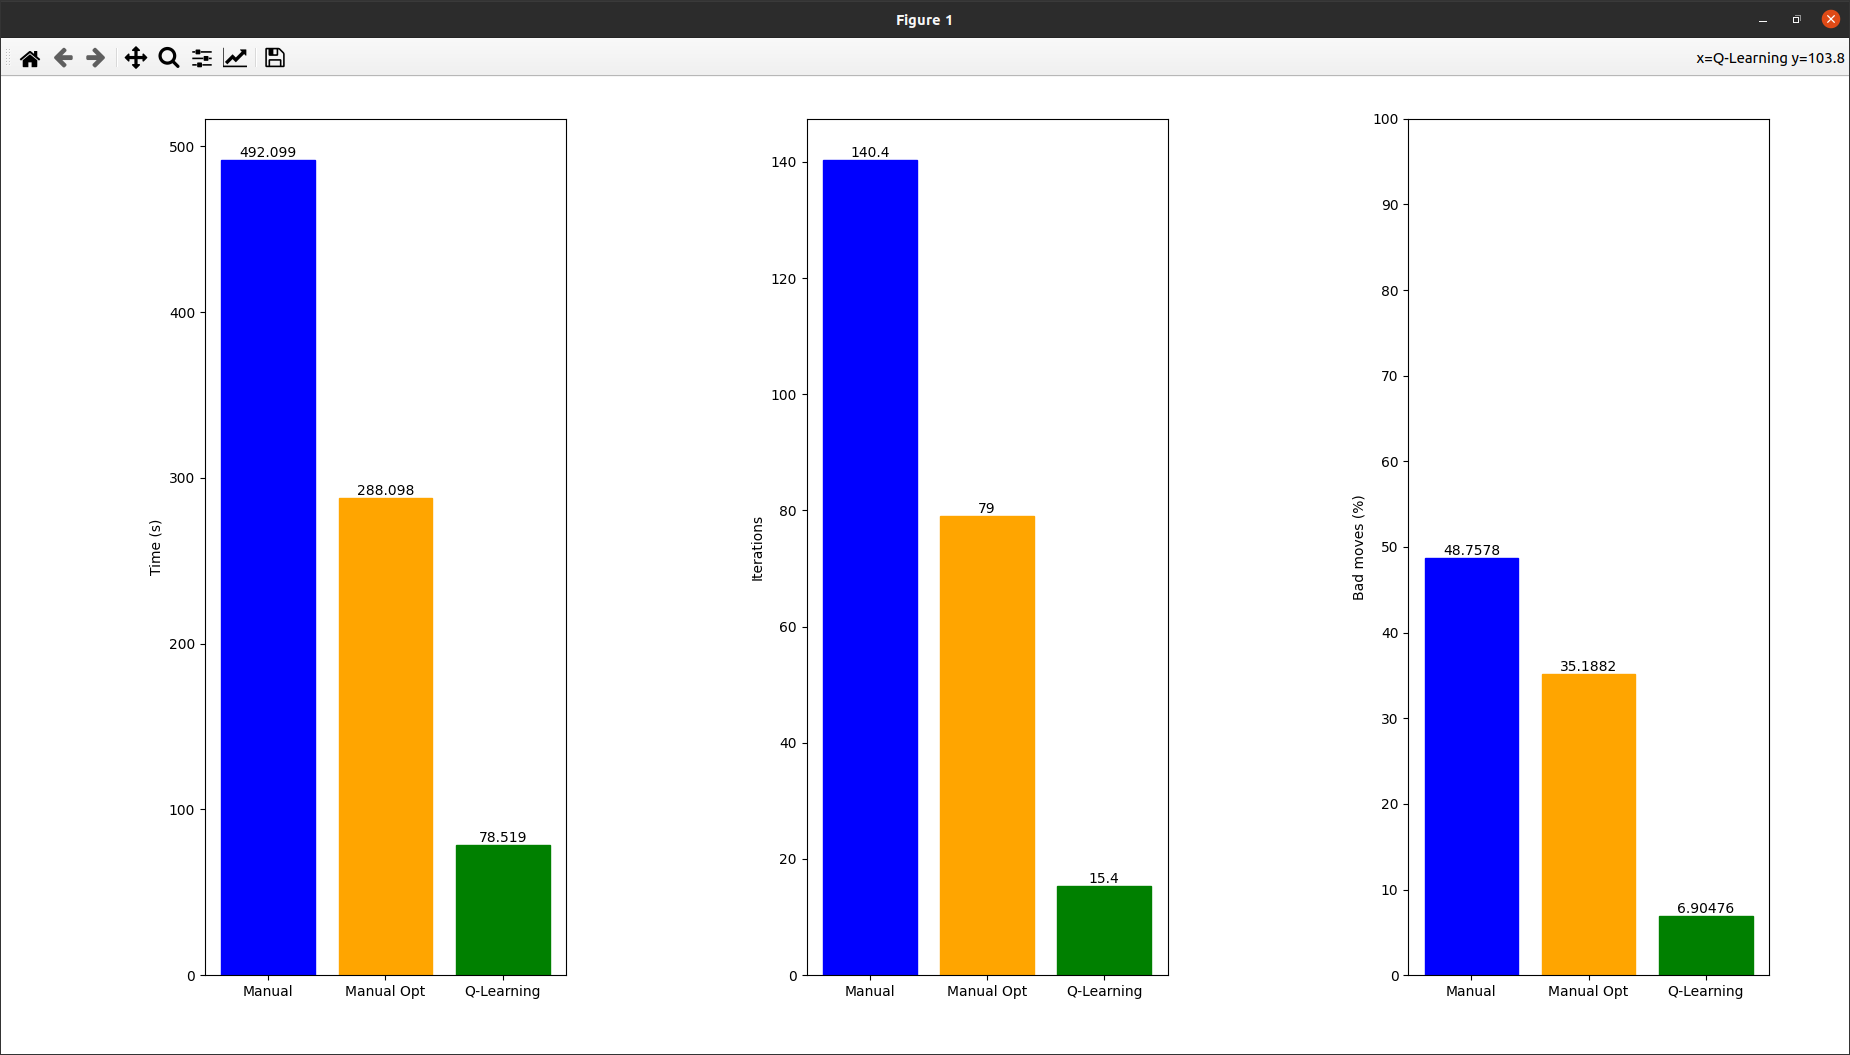
\includegraphics[height=8cm]{imagenes/cap4/24_comp_esq_30.png}
    \end{center}
    \caption[Comparativas (30x30), señal en la esquina]{Comparativas (30x30), señal en la esquina}
    \label{fig:comp_esq_30}
\end{figure}

Finalmente, se ha realizado un experimento sólo para Q-Learning, en el cual se entrena al modelo con una señal, y se realizaba inferencia con otra señal de características distintas, aumentando la potencia del transmisor al doble y cambiando la frecuencia de Wi-Fi a 5G, pero manteniendo las coordenadas en las que se sitúa, que en este caso son (5, 3), lo que se ve en el siguiente mapa de puntos:\\

\begin{figure} [H]
    \begin{center}
    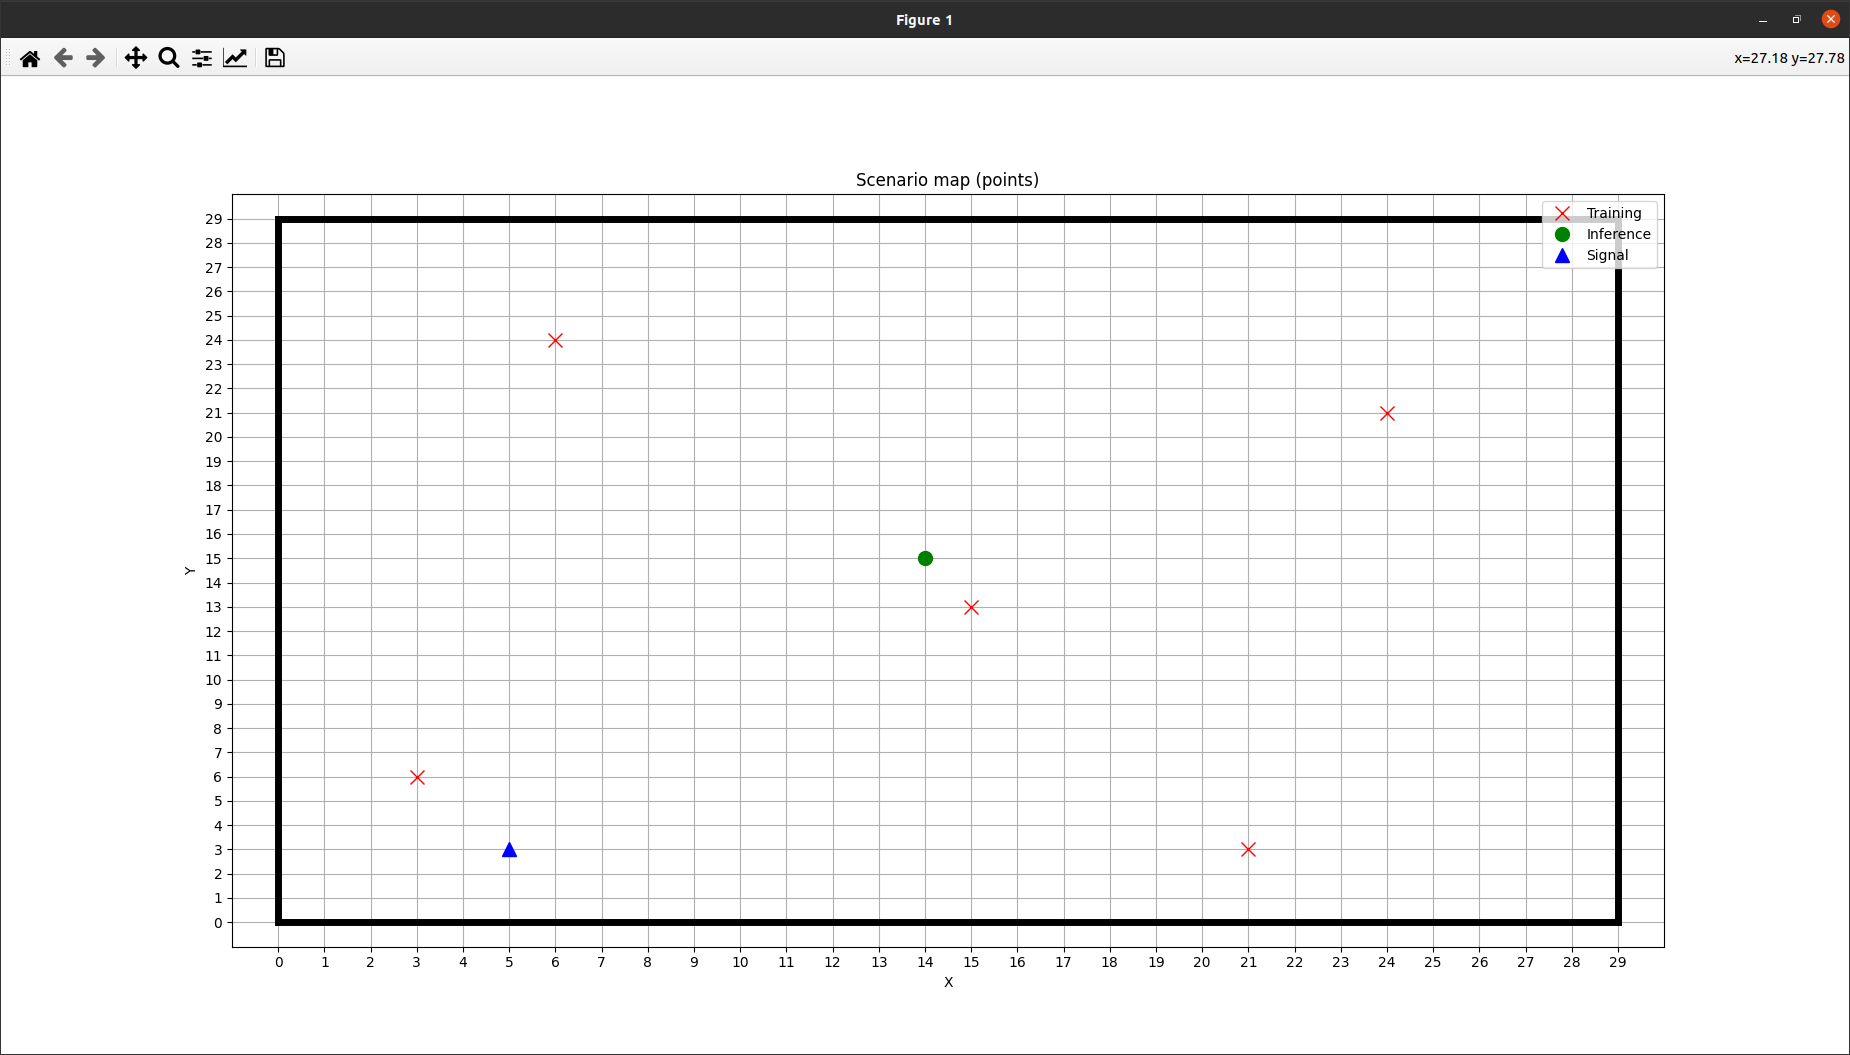
\includegraphics[height=8cm]{imagenes/cap4/25_mapa_p_diff.png}
    \end{center}
    \caption[Mapa de puntos (30x30), señales diferentes]{Mapa de puntos (30x30), señales diferentes}
    \label{fig:map_p_diff_30}
\end{figure}

Para este caso, el problema se resuelve de igual forma para ambos casos, con una cierta variación irrelevante en la métrica temporal, derivada probablemente de la propia simulación:\\

\begin{figure} [H]
    \begin{center}
    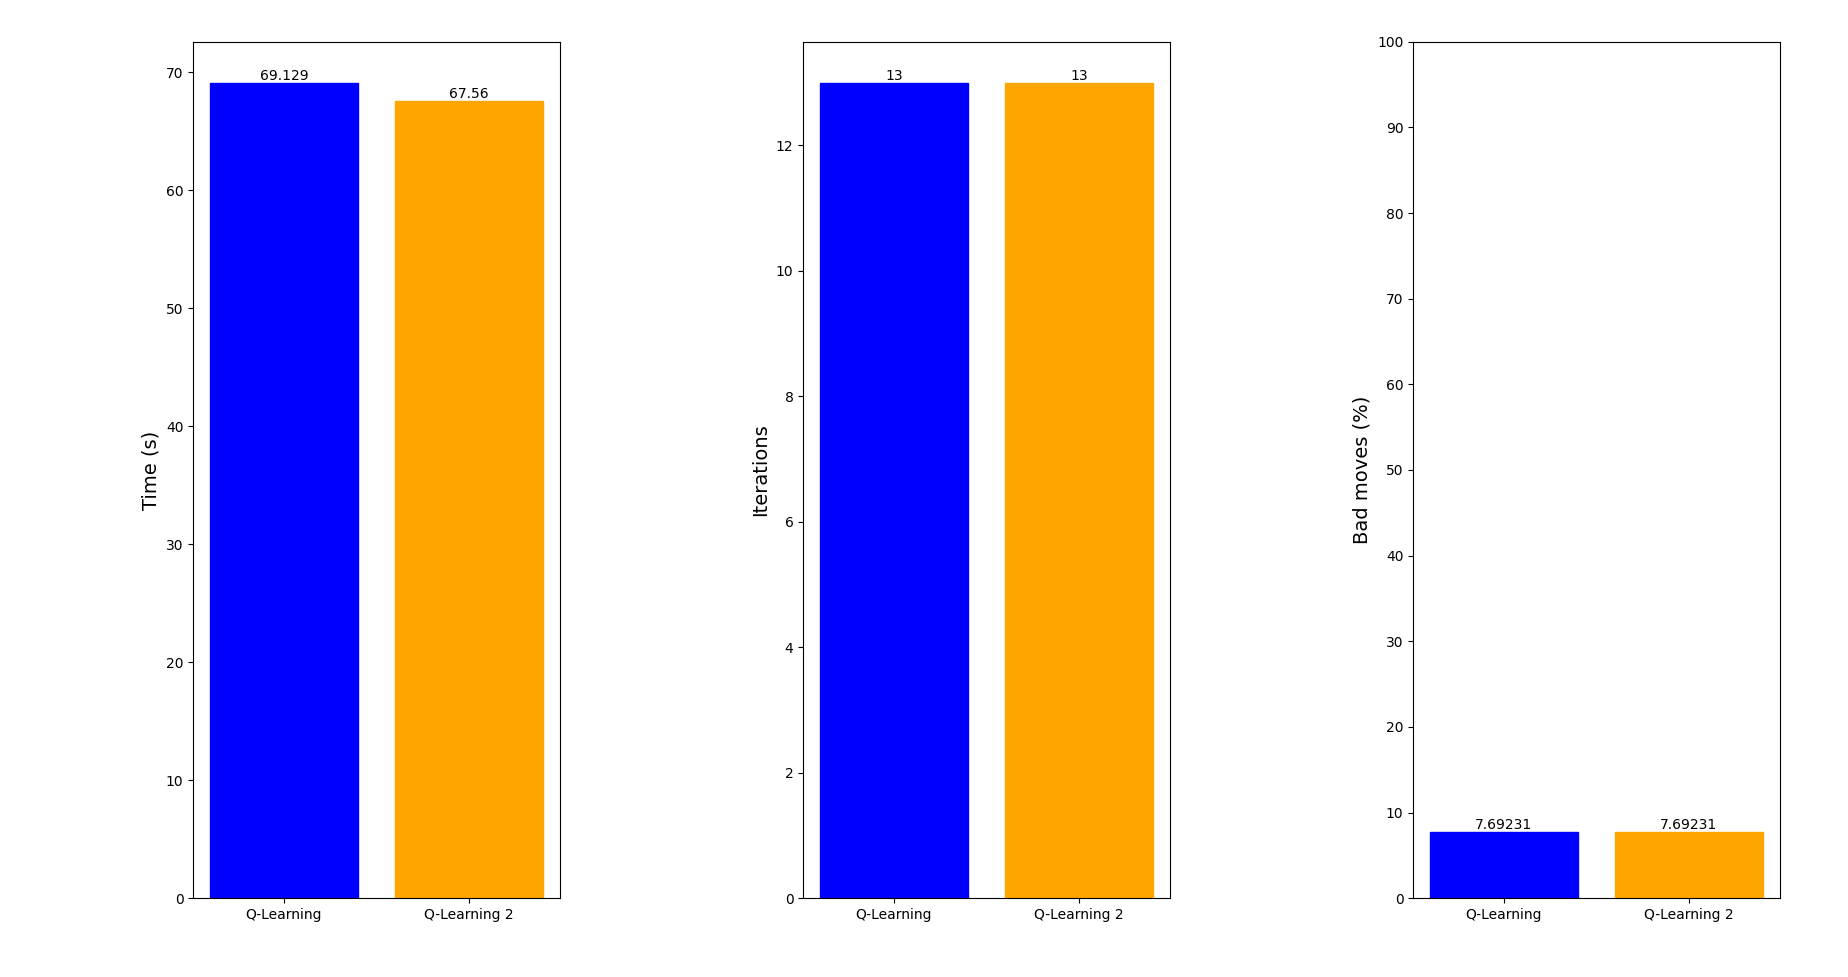
\includegraphics[height=7.5cm]{imagenes/cap4/26_comp_diff.png}
    \end{center}
    \caption[Comparativas (30x30), señales diferentes]{Comparativas (30x30), señales diferentes}
    \label{fig:comp_diff_30}
\end{figure}

\section{Comportamiento sigue señal basado en \ac{RF} en un entorno dinámico}
\label{sec:signal_follow_obs}

\subsection{Introducción al problema}
\label{subsec:intro_sfo}

El escenario planteado anteriormente, es una aproximación poco realista, es decir, en un entorno real se esperan perturbaciones y obstáculos. Por ello, se ha implementado un escenario con muros que distorsionan la señal.\\

Inicialmente, se ha establecido el mapa a mano, es decir, se han sobreescrito los valores degradados de la señal sobre el mapa original para simular un mapa con obstáculos.\\

\subsection{Algoritmos}
\label{subsec:algoritmo_sfo}

En cuanto a los algoritmos empleados, se parte de la idea de realizar un entrenamiento normal sin obstáculos, y ajustar el comportamiento a las situaciones emergentes.\\

Por ello se distinguen dos casos:

\begin{enumerate}
    \item \emph{El dron vuela por encima de la altura del obstáculo}: es decir, el dron navega por una zona con interferencias pero a una altura donde no exista colisión.

    \item \emph{El dron vuela a la misma altura que el obstáculo}: donde según que camino se escoja puede existir colisión.
\end{enumerate}

\subsection{Experimentos y resultados}
\label{subsec:experimentos_sfo}

Por ello, se observa que para el primer caso donde el dron sobrevuela cualquier muro, no existe inconveniente, puesto que el dron toma el camino que tomaría si no hubiera obstáculos. Esto es debido a que en inferencia, tan solo se tiene en cuenta su posición con respecto al mapa de calor, y por tanto no identifica si hay o no obstáculos.\\

En el otro escenario, donde el dron vuela a la altura de los obstáculos, se debe implementar un método de detección de obstáculos. En general, se puede generar un caso realista usando un láser LiDAR o una cámara 3D, pero para simplificar el problema, se ha empleado la información del mapa realizando una simulación del comportamiento que tendría un sensor genérico de este tipo.\\

Por ello, primero se prueba excluyendo las acciones que desemboquen en colisión, donde se presupone que el entrenamiento evitará acciones que alejen al dron de la señal, tal y cómo se observa a continuación:

\begin{figure} [H]
    \begin{center}
    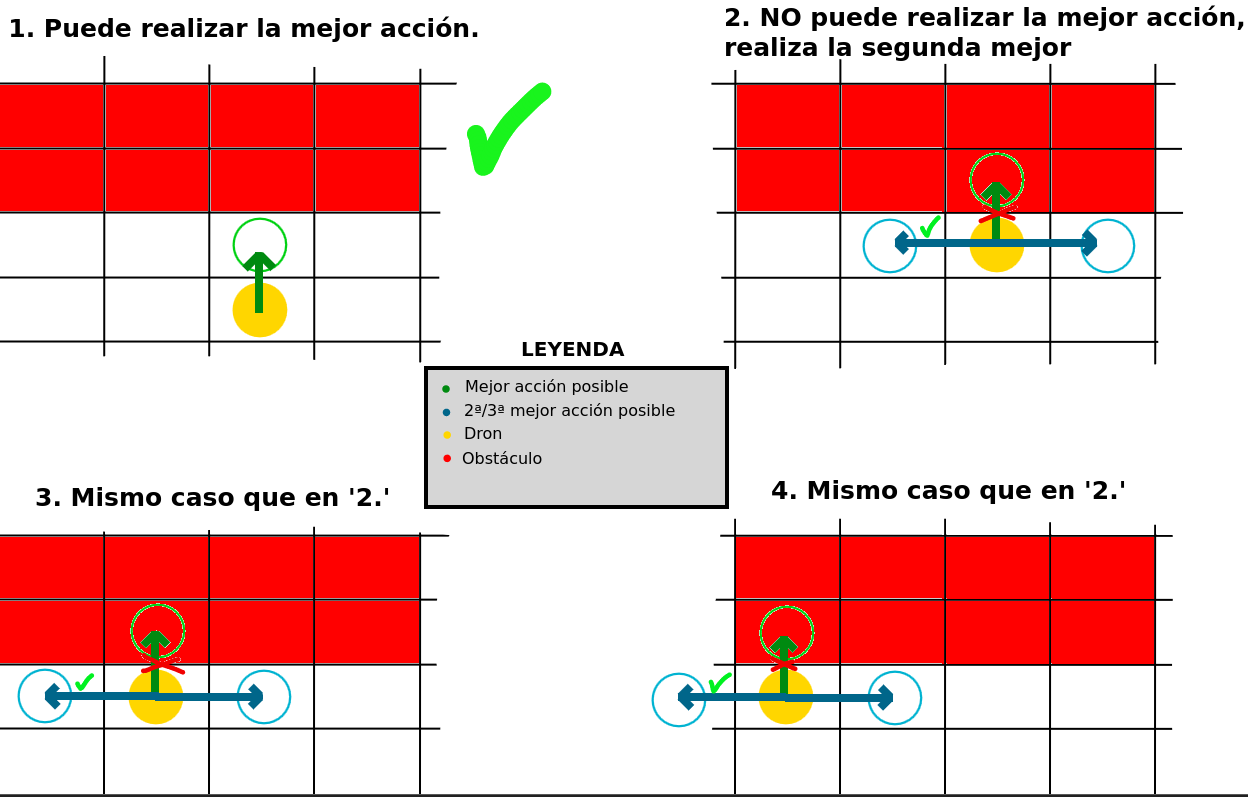
\includegraphics[height=9cm]{imagenes/cap4/28_pseudosensor.png}
    \end{center}
    \caption[Simulación de sensor para obstáculo]{Simulación de sensor para obstáculo}
    \label{fig:pseudosensor}
\end{figure}

Sin embargo, los resultados no son concluyentes, de modo que en ocasiones sortea el obstáculo, pero en otras simplemente retrocede o alcanza un mínimo local.\\

Por ello, y volviendo a la conclusión extraida del primer escenario, se ve la necesidad de aplicar un comportamiento híbrido, de modo que se navegue hacia la señal, hasta topar con un obstáculo lo suficientemente cercano, como para que cambie el modo de actuación para evitarlo. Una vez sorteado, se vuelve modo de navegación normal, hasta llegar a la señal o a otro obstáculo.\\

De este modo, se opta por emplear un algoritmo basado en \ac{VFF}, ... (RELLENAR SI PROCEDE).